%%
%% CSE407 Final Paper - ACM sigconf format
%% Upload the entire paper/ folder to Overleaf, set main.tex as the entry point.
%% Compile: pdflatex -> bibtex -> pdflatex -> pdflatex
%% NOTE: acmart loads natbib internally - biblatex is incompatible. Use BibTeX.
%%
\documentclass[sigconf,nonacm]{acmart}

%% -- Extra packages ---------------------------------------------
\usepackage{booktabs}
\usepackage{array}
\usepackage{microtype}
\usepackage{subcaption}
\usepackage{multirow}
\usepackage{float}   %% enables [H] specifier for exact figure placement

%% ── BibTeX (acmart is incompatible with biblatex) ─────────────
%% The references.bib is authored in BibLaTeX format (url, doi, abstract,
%% eprinttype, urldate fields). BibTeX silently ignores fields it does not
%% understand and processes the standard fields (author, title, year, etc.).

%% ── BibTeX compat shim ────────────────────────────────────────
\AtBeginDocument{%
  \providecommand\BibTeX{{Bib\TeX}}%
  \let\balance\relax}

%% ── Remove all conference / copyright metadata ─────────────────
\setcopyright{none}
\acmYear{2026}
\acmDOI{}
\acmConference[]{}{}{}
\acmISBN{}
\settopmatter{printacmref=false}  %% removes the "ACM Reference Format:" block
\setlength{\headheight}{23.5pt}
\setlength{\emergencystretch}{2em}
\raggedbottom

%% ── Macros ─────────────────────────────────────────────────────
\newcommand{\cmark}{\ensuremath{\checkmark}}
\newcommand{\xmark}{\ensuremath{-}}

\begin{document}

%% ════════════════════════════════════════════════════════════════
%%  TITLE AND AUTHORS
%% ════════════════════════════════════════════════════════════════
\title{Holistic Optimization of Small Language Models for Energy-Efficient Edge Inference: An Empirical Ablation Study}

\author{Md. Sadik Shahriar}
\email{shahriarsadik@gmail.com}
\affiliation{%
  \institution{East West University}
  \department{Department of Computer Science and Engineering}
  \city{Dhaka}
  \country{Bangladesh}}

\author{Nipa Mridha}
\email{mridhanipa886@gmail.com}
\affiliation{%
  \institution{East West University}
  \department{Department of Computer Science and Engineering}
  \city{Dhaka}
  \country{Bangladesh}}

\author{Tanha Humaira}
\email{chandnihumaira373@gmail.com}
\affiliation{%
  \institution{East West University}
  \department{Department of Computer Science and Engineering}
  \city{Dhaka}
  \country{Bangladesh}}

\renewcommand{\shortauthors}{Shahriar, Mridha, and Humaira}

%% ════════════════════════════════════════════════════════════════
%%  ABSTRACT
%% ════════════════════════════════════════════════════════════════
\begin{abstract}
Deploying small language models (SLMs) on power-constrained edge hardware requires balancing energy consumption, memory footprint, decode throughput, and task accuracy. While individual compression techniques (such as 4-bit weight quantization, token eviction, and KV-cache quantization) are typically developed and evaluated in isolation or algorithmic simulation, real-world edge systems frequently stack these techniques sequentially. This paper presents an empirical systems study evaluating the physical interactions, operational boundaries, and software-to-hardware realization gaps of stacked compression pipelines on an NVIDIA T4 GPU across context lengths of 1024, 2048, and 4096 tokens, continuously sampling board power at 10~Hz via NVML. Retrieval fidelity is assessed using a calibrated 60-scenario hard-retrieval benchmark requiring exact-match key-value extraction from 4096-token documents across three document depths.

Our measurements demonstrate that compression efficiency and heuristic stability are strictly governed by attention geometry and sequence length rather than nominal compression ratios alone. On Llama~3.2-3B (3:1 GQA), stacking 4-bit AWQ with custom PyramidKV eviction establishes the optimal empirical frontier at 4096 tokens: reducing total energy consumption by 101.95~J (16.15\%), shrinking active KV cache storage by 73.8\% (from 455~MiB to 119~MiB), and accelerating decode throughput by 47.7\% (from 13.77 to 20.34~tok/s) while preserving accuracy (37/60 vs.\ 38/60 baseline). In stark contrast, applying the identical eviction policy to Qwen2.5-3B (8:1 GQA) causes hard-retrieval accuracy to collapse from 48/60 to 1/60, a failure that persists even after expanding the retention budget by 50\% (2/15 recovered). We also formally prove and measure a statistically significant compound shielding effect ($I < 0, p < 0.01$), where prior token eviction reduces the computational and memory bandwidth workload of downstream quantization routines. Finally, we quantify a substantial software-to-hardware realization gap in off-the-shelf reference quantization packages that eagerly retain uncompressed state. These empirical findings provide hardware-grounded boundary conditions for theoretical rate-distortion frameworks, such as ThinKV and RDKV, and provide actionable guidelines for edge system architects.
\end{abstract}

%% ── Keywords ───────────────────────────────────────────────────
\keywords{Green AI, energy-efficient inference, KV cache compression, token
eviction, weight quantization, AWQ, TurboQuant, PyramidKV, small language models,
edge deployment, NVIDIA T4, needle-in-a-haystack}

\maketitle

%% ════════════════════════════════════════════════════════════════
%%  1. INTRODUCTION
%% ════════════════════════════════════════════════════════════════
\section{Introduction}

Deploying language models on power-constrained edge accelerators requires balancing energy consumption, memory footprint, decode throughput, and task accuracy~\cite{strubell_energy_2019,patterson_carbon_2021,schwartz2020green}. As language processing workloads shift toward local micro-servers and embedded accelerators, the memory bandwidth required by the Key-Value (KV) cache becomes the primary operational bottleneck~\cite{li2024survey}.

During autoregressive generation, transformers store past key and value vectors for every processed token. This cache grows linearly with sequence length. Because every newly decoded token requires loading the entire accumulated KV cache from DRAM, inference on bandwidth-limited edge hardware, such as the NVIDIA T4 (the standard micro-server baseline with a 70~W enforced power limit), becomes strictly memory bound during decoding. Small language models (SLMs) with sub-4B parameters offer a practical footprint for edge use cases~\cite{husom_sustainable_2025}. However, their physical energy scaling under multi-stage compression remains poorly characterized. Many compression studies evaluate individual techniques in isolation, rely on FLOP-based analytical models, or study large server-scale models with attention dynamics that differ fundamentally from compact edge SLMs~\cite{wang_slmquant_2025}.

To reduce memory traffic during generation, researchers have explored three primary compression paradigms:
\begin{itemize}\raggedright
  \item \textbf{Weight Quantization} (e.g., AWQ~\cite{lin_awq_2025}) compresses model parameters to low bit-widths (such as 4 bits), reducing static model memory and weight transfer during prefill and decode.
  \item \textbf{Token Eviction} (e.g., PyramidKV~\cite{cai_pyramidkv_2025}, SnapKV~\cite{li_snapkv_2024}, H2O~\cite{zhang_h2o_2023}) prunes uninformative tokens from the cache based on attention scores, shrinking both the active memory footprint and dynamic memory read traffic during decoding.
  \item \textbf{KV-Cache Quantization} (e.g., TurboQuant~\cite{zandieh2026turboquant}, KIVI~\cite{liu_kivi_2023}, JanusQuant~\cite{sun2026janusquant}) reduces the numerical precision of cached vectors to decrease byte usage per retained token.
\end{itemize}

Recent theoretical studies have proposed uniting token pruning with precision reduction. Frameworks like \textbf{RDKV}~\cite{zhang_rdkv_2026} formulate joint KV-cache compression using rate-distortion theory via reverse water-filling bit allocation, while \textbf{ThinKV}~\cite{ramachandran_thinkv_2026} develops dynamic token and bit allocation for reasoning trajectories. Although these formulations present compelling trade-offs in algorithmic simulation, physical hardware data on multi-stage compression on sub-4B models remains scarce. Systems practitioners currently lack empirical evidence on how independently implemented compression tools behave when stacked together sequentially, how attention head-sharing affects pruning reliability, and how much runtime overhead arises in physical deployment.

This paper presents an empirical systems study of these multi-stage interactions on physical silicon. We evaluate the sequential composition of AWQ 4-bit weight quantization, custom PyramidKV-style token eviction, and TurboQuant KV-cache quantization on two representative 3B-parameter models (Llama~3.2-3B-Instruct and Qwen2.5-3B-Instruct) on an NVIDIA T4 GPU, logging board-level power continuously at 10~Hz via NVML.

\paragraph{Research Questions.}
We investigate four core questions:
\begin{enumerate}
  \item \textbf{RQ1 (Context Scaling and Multi-Stage Efficiency):} How do weight quantization, token eviction, and KV-cache quantization individually and sequentially affect physical GPU energy consumption and throughput across sequence lengths of 1024, 2048, and 4096 tokens?
  \item \textbf{RQ2 (Cross-Architectural Robustness):} Does token eviction provide consistent trade-offs across different attention layouts (Llama's 3:1 vs.\ Qwen's 8:1 GQA), or does aggressive head sharing cause retrieval failures?
  \item \textbf{RQ3 (Compound Interaction and Overhead Shielding):} When multiple compression stages are applied sequentially, do they compound additively or exhibit energetic shielding interactions?
  \item \textbf{RQ4 (Multi-Objective Pareto Optimization):} Which compression combinations form the non-dominated Pareto frontier when energy, retrieval accuracy, and persistent memory footprint are evaluated under bootstrap resampling?
\end{enumerate}

\paragraph{Key Contributions.}
The contributions of this work are:
\begingroup\raggedright
\begin{enumerate}
  \item \textbf{Hardware-Grounded Empirical Baselines:} We provide direct 10~Hz NVML physical energy measurements across two 3B models, three context lengths, and five compression configurations, establishing physical silicon baselines that ground theoretical joint compression models (such as RDKV and ThinKV).
  \item \textbf{Cross-Architectural Eviction Sensitivity:} We identify a 76.7 percentage-point cross-model accuracy difference under token eviction. Eviction performs well on balanced GQA (Llama: 16.15\% energy reduction, 47.7\% throughput increase, 73.8\% memory reduction, and 37/60 vs.\ 38/60 baseline retrieval), but collapses under aggressive 8:1 GQA (Qwen: 1/60 retrieval), showing that GQA head sharing is a critical operational boundary.
  \item \textbf{Compound Overhead Shielding:} We measure and statistically verify a negative interaction contrast ($I < 0, p < 0.01$) on both models, demonstrating that pruning tokens prior to quantization acts as an energy shield that reduces the data volume handled by subsequent quantization routines.
  \item \textbf{Calibrated Benchmark and Pareto Analysis:} We design a calibrated 4096-token hard-retrieval benchmark (developed across four pilot iterations) and build a 3-objective Pareto frontier evaluated over 2000 bootstrap resamples with power capping checks.
\end{enumerate}
\endgroup


%% ════════════════════════════════════════════════════════════════
%%  2. RELATED WORK
%% ════════════════════════════════════════════════════════════════
\section{Related Work}

\subsection{Weight Quantization}
Weight quantization compresses floating-point model parameters into low-bit integers, reducing memory footprint and parameter transfer bandwidth. AWQ~\cite{lin_awq_2025} identifies activation-salient weight channels and protects them from quantization error during 4-bit compression. GPTQ~\cite{frantar_gptq_2023} uses layer-wise second-order error compensation. For compact models, SLMQuant~\cite{wang_slmquant_2025} showed that sub-4B architectures are more sensitive to aggressive quantization than larger models. This sensitivity highlights the need for direct hardware evaluation on specific SLMs rather than assuming trends from large-scale LLMs hold.

\subsection{Token Eviction}
Token eviction reduces KV-cache memory by pruning uninformative tokens during generation. H2O~\cite{zhang_h2o_2023} showed that retaining a small fraction (roughly 20\%) of accumulated attention recipients (termed ``heavy hitters'') preserves most generative capability. SnapKV~\cite{li_snapkv_2024} identifies important tokens using an observation window over recent prompt positions. PyramidKV~\cite{cai_pyramidkv_2025} refines this by assigning layer-dependent budgets: deeper layers retain more tokens while shallower layers retain fewer, improving long-context retrieval accuracy by 5\% to 15\% over uniform budgets.

\subsection{KV-Cache Quantization}
KV-cache quantization reduces the numerical precision of stored key and value vectors. TurboQuant~\cite{zandieh2026turboquant} applies random orthogonal rotations to KV vectors followed by scalar quantization without requiring calibration data. KIVI~\cite{liu_kivi_2023} uses per-channel key and per-token value quantization at 2-bit precision. Salfati et al.~\cite{salfati_quantization_2026} demonstrated that uniform quantization preserves attention score rankings better than low-rank approximations, particularly for grouped-query attention (GQA) architectures. Sun et al.~\cite{sun2026janusquant} introduced JanusQuant for long-context 2-bit quantization.

\subsection{Joint and Compound Compression}
Recent theoretical work investigates combining token pruning with precision reduction. RDKV~\cite{zhang_rdkv_2026} frames KV-cache compression as a rate-distortion optimization problem, jointly determining token retention and bit allocation through reverse water-filling. ThinKV~\cite{ramachandran_thinkv_2026} allocates tokens and precision dynamically for reasoning models. While these methods demonstrate promising accuracy-memory trade-offs in simulation, neither reports physical energy measurements on sub-4B models. Our C4-Ref setting evaluates sequential stacking (eviction followed by quantization) on physical hardware, providing an empirical baseline for joint compression strategies.

\subsection{Energy Measurement in LLM Inference}
Argerich et al.~\cite{argerich_watt_2026} evaluated over 5,000 inference runs and found that 10~Hz NVML power sampling offers an accurate, low-overhead measurement of GPU energy. They measured NVIDIA T4 idle power at approximately 12~W and peak operating power near 82~W. Husom et al.~\cite{husom_sustainable_2025} measured quantized SLMs on edge platforms, showing that energy scaling varies by sequence length and workload. We adopt their measurement protocols.

\subsection{Taxonomy of Related Work}

Table~\ref{tab:comparison} compares our work with prior literature across weight quantization, token eviction, KV quantization, and hardware energy measurement.

\begin{table}[htbp]
\caption{Coverage Comparison with Related Work}
\label{tab:comparison}
\centering\small
\begin{tabular}{lcccc}
\toprule
\textbf{Work} & \textbf{Wt.Q} & \textbf{Evict} & \textbf{KVQ} & \textbf{Energy} \\
\midrule
AWQ~\cite{lin_awq_2025}            & \cmark & \xmark & \xmark & \xmark \\
GPTQ~\cite{frantar_gptq_2023}      & \cmark & \xmark & \xmark & \xmark \\
SLMQuant~\cite{wang_slmquant_2025} & \cmark & \xmark & \xmark & \xmark \\
H2O~\cite{zhang_h2o_2023}        & \xmark & \cmark & \xmark & \xmark \\
SnapKV~\cite{li_snapkv_2024}     & \xmark & \cmark & \xmark & \xmark \\
PyramidKV~\cite{cai_pyramidkv_2025}& \xmark & \cmark & \xmark & \xmark \\
TurboQuant~\cite{zandieh2026turboquant} & \xmark & \xmark & \cmark & \xmark \\
KIVI~\cite{liu_kivi_2023}          & \xmark & \xmark & \cmark & \xmark \\
RDKV~\cite{zhang_rdkv_2026}        & \xmark & \cmark & \cmark & \xmark \\
ThinKV~\cite{ramachandran_thinkv_2026} & \xmark & \cmark & \cmark & \xmark \\
Watt Counts~\cite{argerich_watt_2026} & \xmark & \xmark & \xmark & \cmark \\
\textbf{This Work}                 & \cmark & \cmark & \cmark & \cmark \\
\bottomrule
\end{tabular}
\end{table}


%% ════════════════════════════════════════════════════════════════
%%  3. METHODOLOGY
%% ════════════════════════════════════════════════════════════════
\section{Methodology}

Figure~\ref{fig:methodology} illustrates our experimental workflow, including model configurations, power sampling, quality evaluation, and statistical analysis.

\begin{figure*}[htbp]
\centering
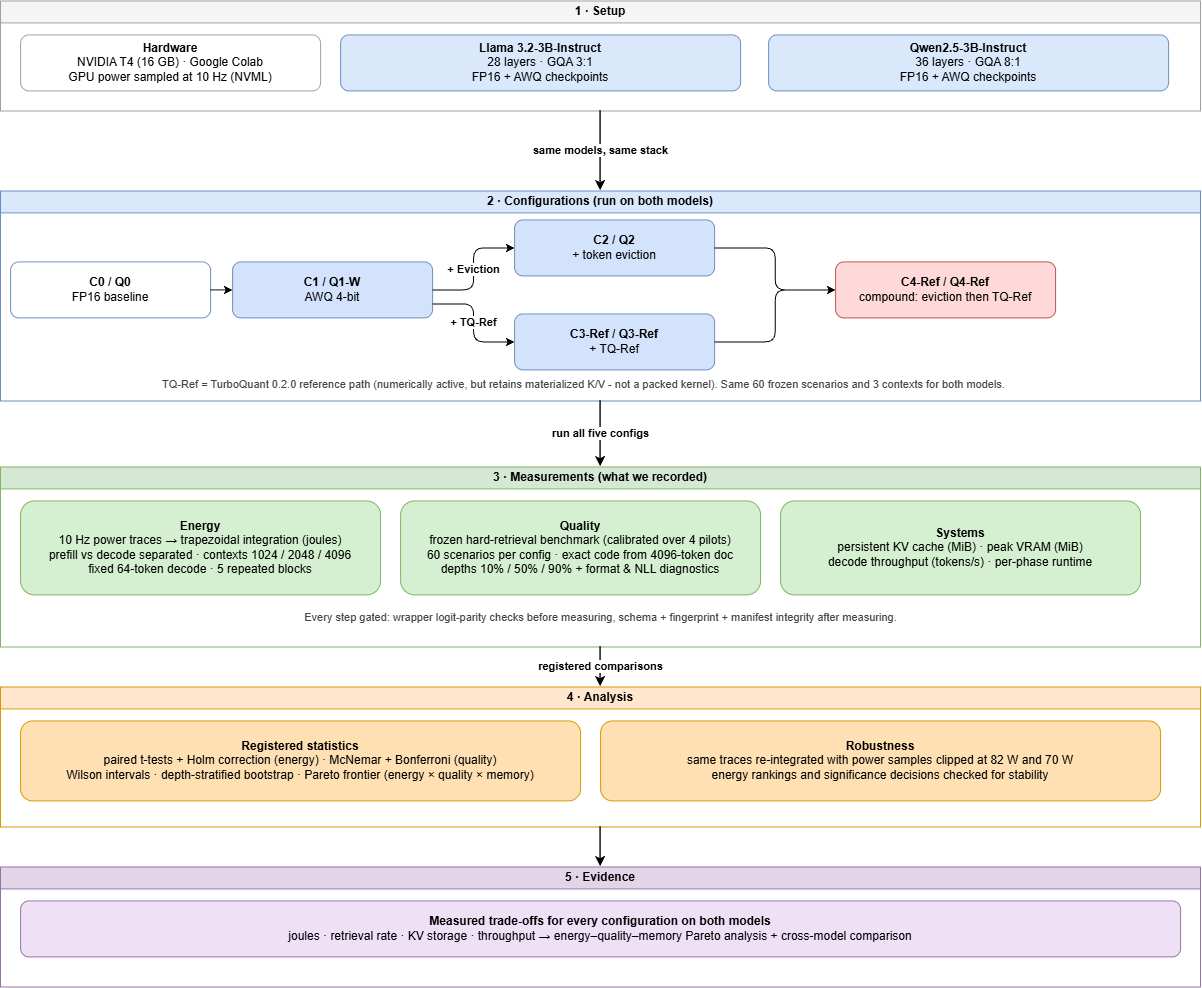
\includegraphics[width=\textwidth]{figures/methodology_diagram.png}
\Description{A flowchart summarizes the experiment: five compression configurations are evaluated on Llama 3.2-3B and Qwen2.5-3B, then power, retrieval, and system metrics are analyzed statistically and under power caps.}
\caption{Experimental methodology flowchart. The pipeline evaluates five compression configurations on Llama 3.2-3B and Qwen2.5-3B, logging 10~Hz power traces, hard-retrieval quality, and system trade-offs, followed by statistical and power-robustness checks.}
\label{fig:methodology}
\end{figure*}

\subsection{Model Architectures}

We evaluate two open-weight 3B-parameter models. Table~\ref{tab:geometry} lists their architectural parameters. The models differ in layer count, native context window, and Grouped-Query Attention (GQA)~\cite{ainslie2023gqa} configuration. Qwen uses an 8:1 GQA ratio (16 query heads sharing 2 KV heads), while Llama uses a 3:1 ratio (24 query heads sharing 8 KV heads).

\begin{table}[htbp]
\caption{Model Architecture Specifications}
\label{tab:geometry}
\centering\small
\begin{tabular}{lrr}
\toprule
\textbf{Property} & \textbf{Llama 3.2-3B} & \textbf{Qwen2.5-3B} \\
\midrule
Layers              & 28  & 36  \\
Query heads         & 24  & 16  \\
KV heads            & 8   & 2   \\
GQA ratio           & 3:1 & 8:1 \\
Head dimension      & 128 & 128 \\
Native context      & 8K  & 32K \\
\bottomrule
\end{tabular}
\end{table}

For Llama, we used the Unsloth Llama-3.2-3B-Instruct checkpoint~\cite{unsloth_2024} for the FP16 baseline and the CasperHansen AWQ release~\cite{casperhansen_llama32_awq} for 4-bit weights. For Qwen, we used the official Qwen2.5-3B-Instruct checkpoints~\cite{qwen2024technical}. All revisions are recorded in the experiment registry. The software environment used PyTorch~2.11.0~\cite{paszke2019pytorch}, Transformers~5.12.1~\cite{wolf2020transformers}, and TurboQuant~0.2.0~\cite{zandieh_turboquant_v020}.

\subsection{Experimental Configurations}

We define five configurations to evaluate individual and combined compression effects:

\begin{table}[htbp]
\caption{Core Compression Configurations}
\label{tab:configs}
\centering\small
\resizebox{\columnwidth}{!}{%
\begin{tabular}{@{}lllll@{}}
\toprule
\textbf{Config} & \textbf{Llama} & \textbf{Qwen} & \textbf{Weights} & \textbf{KV Compression} \\
\midrule
FP16 baseline   & C0    & Q0    & FP16      & None \\
AWQ baseline    & C1/C1-W & Q1-W & AWQ 4-bit & None \\
Eviction        & C2    & Q2    & AWQ 4-bit & PyramidKV-style token eviction \\
TQ-Ref only     & C3-Ref & Q3-Ref & AWQ 4-bit & TurboQuant numerical reference \\
Compound        & C4-Ref & Q4-Ref & AWQ 4-bit & Eviction \emph{then} TQ-Ref \\
\bottomrule
\end{tabular}}
\end{table}

Each configuration targets a specific component in the inference pipeline:
\begin{itemize}
  \item \textbf{C0 / Q0 (FP16 Baseline):} Uncompressed model execution, providing baseline values for memory allocation, power draw, and full-precision retrieval accuracy.
  \item \textbf{C1 / Q1-W (AWQ Baseline):} 4-bit weight-only quantization, measuring parameter memory reduction and bandwidth savings without altering the KV cache.
  \item \textbf{C2 / Q2 (PyramidKV Eviction):} AWQ combined with layerwise token eviction (averaging 1024 retained tokens per layer), testing whether spatial pruning reduces decode memory traffic while retaining retrieval capability.
  \item \textbf{C3-Ref / Q3-Ref (TurboQuant Reference):} AWQ combined with numerical KV-cache quantization, measuring numerical retrieval accuracy alongside the runtime overhead of the reference package.
  \item \textbf{C4-Ref / Q4-Ref (Sequential Compound):} All three techniques stacked sequentially (AWQ $\to$ eviction $\to$ TurboQuant), testing whether multi-stage compression delivers compounding energy savings or exhibits interaction effects.
\end{itemize}

We also ran two sensitivity sweeps at 4096 tokens: eviction budget (512, 1024, and 1536 average retained tokens per layer) and TurboQuant nominal precision (2, 3, and 4 bits).

\subsection{Hardware and Power Measurement Protocol}

Experiments ran on an NVIDIA T4 GPU (16~GB nominal VRAM) in Google Colab. We polled GPU board power at 10~Hz (100~ms intervals) through NVML~\cite{nvidia2024nvml} using \texttt{pynvml}, following the methodology of Argerich et al.~\cite{argerich_watt_2026}. Total energy in Joules was computed via trapezoidal numerical integration over the recorded power trace, with prefill and decode phases integrated separately.

To isolate compression effects from variations in autoregressive text generation, all energy runs used teacher-forced decoding for exactly 64 tokens. This keeps token generation identical across configurations, ensuring that measured energy differences reflect only the compression mechanism. We tested three context lengths (1024, 2048, and 4096 tokens) with five independent measurement blocks per condition. For each run, we logged power traces, timestamps, clock frequencies, board temperatures, and allocated VRAM.

\subsection{Eviction Implementation}

We implement token eviction using a custom attention wrapper. During prefill, token importance scores are computed by averaging attention weights over a 32-token observation window. We apply a layer-dependent pyramidal budget averaging 1024 retained tokens per layer (allocating larger budgets to deeper layers and smaller budgets to shallower layers). Tokens below the layer threshold are evicted from the active cache before decoding begins. We validated this wrapper on Qwen's 8:1 GQA layout before collecting primary benchmark data (Section~\ref{sec:qwen-energy}).

\subsection{TurboQuant Reference Implementation and Realization Audit}

TurboQuant~\cite{zandieh2026turboquant} applies random orthogonal rotations to KV vectors and maps coordinates to discrete codebook indices. We evaluate the public reference package, version~0.2.0~\cite{zandieh_turboquant_v020}. In this reference implementation, coordinates are stored as \texttt{uint8} indices while uncompressed FP16 key and value tensors remain concurrently allocated in memory. Consequently, the reference path is numerically active (applying quantized representations during attention computation) but does not compress physical memory on device because uncompressed tensors are retained. Nominal bit widths (2, 3, or 4 bits) adjust codebook quantization levels without changing physical container byte allocation.

Rather than assessing an idealized hardware kernel, evaluating this path serves as an empirical audit of the \emph{software-to-hardware realization gap}: the disconnect between theoretical compression formulations and how off-the-shelf libraries execute on silicon when imported by edge practitioners. To guide future kernel engineering, we formulate a symbolic energy break-even boundary (Appendix~\ref{app:ideal}) specifying the exact compute-overhead thresholds ($O_\text{net} < \epsilon_\text{mem} \cdot \Delta_D$) that a custom packed and fused CUDA/Triton kernel must satisfy to deliver net energy reductions.

\subsection{Statistical Methodology}

Energy differences are evaluated using paired two-sided $t$-tests across the five measurement blocks ($n=5$), reporting 95\% confidence intervals and controlling family-wise error rates with Holm sequential step-down correction~\cite{holm1979simple}. Non-parametric Wilcoxon signed-rank tests~\cite{wilcoxon1945individual} serve as secondary verification. Retrieval accuracy across the 60 benchmark scenarios is reported with Wilson score 95\% confidence intervals~\cite{wilson1927probable}, and paired binary accuracy differences are tested using exact McNemar tests~\cite{mcnemar1947note} with Bonferroni correction. Cross-model retrieval contrasts are estimated with depth-stratified bootstrap resampling (2000 iterations), and Pareto frontier stability is evaluated across 2000 bootstrap resamples.


%% ════════════════════════════════════════════════════════════════
%%  4. DESIGNING THE HARD-RETRIEVAL BENCHMARK
%% ════════════════════════════════════════════════════════════════
\section{Designing the Diagnostic Retrieval Benchmark}
\label{sec:benchmark}

Evaluating KV-cache compression requires a quality metric that directly isolates representational loss in the memory cache. Standard downstream NLP benchmarks (such as multiple-choice QA or sentiment classification) predominantly probe static parameter knowledge rather than long-context memory retention. Furthermore, naive synthetic needle-in-a-haystack (NIAH) benchmarks~\cite{kamradt2023needle} insert a single unstructured fact into natural prose; in our preliminary trials on Llama, all five compression configurations achieved 100\% retrieval accuracy on naive NIAH prompts, creating an uninformative ceiling effect that masked differences between configurations.

\subsection{Benchmark Calibration Principle}

Following the evaluation methodology established in KV-cache compression literature (e.g., SnapKV~\cite{li_snapkv_2024}, PyramidKV~\cite{cai_pyramidkv_2025}, and H2O~\cite{zhang_h2o_2023}), we constructed a calibrated key-value retrieval benchmark. The model must locate a specific target record within a 4096-token synthetic document and extract the associated code following a strict formatting template. The target needle is placed at one of three document depths: beginning (10\%), middle (50\%), or end (90\%).

Calibrating task difficulty is essential: excessive distractor similarity causes baseline failure (floor effects), whereas an overly simple task masks compression degradation (ceiling effects). We calibrated distractor density and key distinctiveness so the uncompressed baseline achieves high but imperfect accuracy ($\approx 75\%-88\%$), leaving headroom to detect compression degradation. The four pilot calibration iterations (V1 to V4) are documented in Appendix~\ref{app:benchmark-pilots}.

\subsection{Frozen Benchmark Specification}

The frozen benchmark uses 60 scenarios per configuration (20 scenarios at each of the 10\%, 50\%, and 90\% depth levels). Each prompt is created using the model's native tokenizer and chat template, then filled with structured distractors to reach exactly 4096 tokens.

Figure~\ref{fig:hard_retrieval} illustrates the document structure. Evaluation requires exact-match extraction of both the target key and the requested return value. We record semantic retrieval accuracy and format compliance separately, with retrieval accuracy serving as the primary quality metric.

\begin{figure*}[!t]
\centering
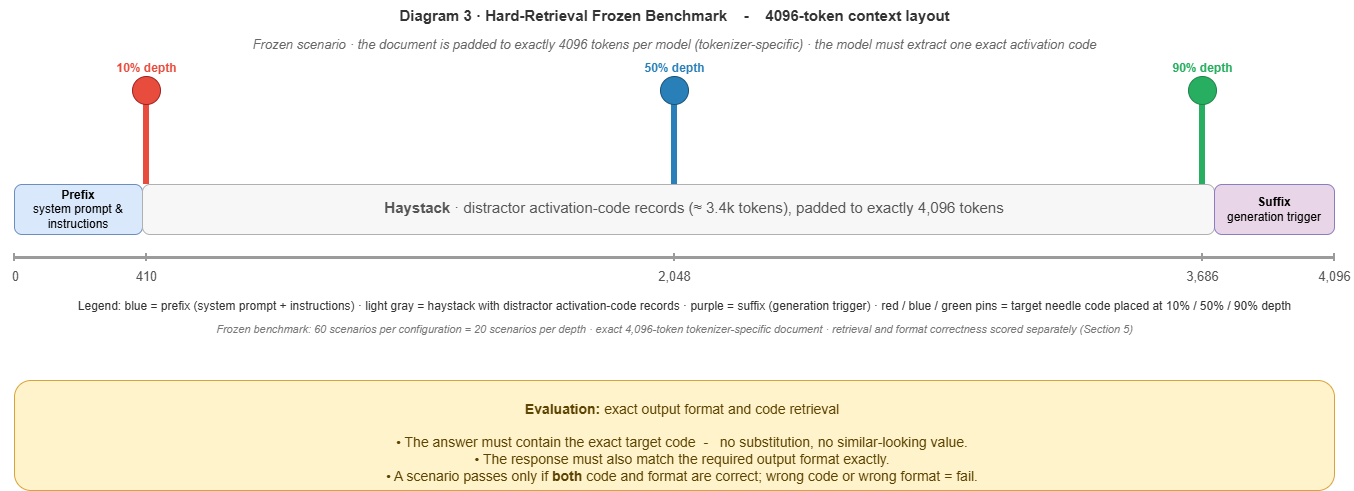
\includegraphics[width=0.98\textwidth]{figures/hard_retrieval.png}
\Description{A 4096-token document diagram shows target-code needles inserted at 10, 50, and 90 percent depth within distractor text, with strict exact-match evaluation.}
\caption{Overview of the 4096-token frozen hard-retrieval benchmark, illustrating the 10\%, 50\%, and 90\% depth needle insertion points within the distractor haystack, and the strict evaluation criteria.}
\label{fig:hard_retrieval}
\end{figure*}


%% ════════════════════════════════════════════════════════════════
%%  5. RESULTS
%% ════════════════════════════════════════════════════════════════
\section{Results}

We present our experimental findings across three domains: hardware energy and decode throughput scaling, sequential interaction and memory trade-offs, and hard-retrieval quality with multi-objective Pareto analysis.

\subsection{TurboQuant Reference Energy Overhead by Phase}

Table~\ref{tab:llama-all} and Table~\ref{tab:qwen-all} report the physical energy overhead of the TurboQuant reference path during prefill and decode. Across all tested contexts, the reference package increases net energy consumption. Decode energy overhead grows with sequence length, exceeding 80\% for Llama TQ-only at 4096 tokens, because autoregressive decoding repeatedly reads uncompressed tensor structures from memory. When eviction precedes quantization, the smaller cache volume reduces the data handled by reference routines, partially mitigating this overhead (Section~\ref{sec:interaction}). A complete breakdown of prefill versus decode overhead across all sequence lengths is plotted in Appendix~\ref{app:context-scaling} (Figure~\ref{fig:tq-overhead}).

\subsection{Llama: Energy Across Context Lengths}
\label{sec:llama-energy}

Table~\ref{tab:llama-all} summarizes measured energy, decode throughput, peak allocated VRAM, and active KV cache volume for Llama~3.2-3B across all three context lengths. Scaling curves are shown in Appendix~\ref{app:context-scaling} (Figure~\ref{fig:context-scaling}).

\begin{table}[htbp]
\caption{Llama Energy (J, mean $\pm$ SD) and Throughput Across Contexts}
\label{tab:llama-all}
\centering\small
\resizebox{\columnwidth}{!}{%
\begin{tabular}{@{}lrrrr@{}}
\toprule
\textbf{Config@Context} & \textbf{Total J} & \textbf{tok/s} & \textbf{Peak VRAM (MiB)} & \textbf{Cache (MiB)} \\
\midrule
C0 @ 1024   & $244.11 \pm 13.10$ & 21.09 & 8810 & 119 \\
C1 @ 1024   & $268.77 \pm 26.20$ & 18.24 & 4943 & 119 \\
C2 @ 1024   & $253.61 \pm 14.36$ & 19.31 & 4920 & 92  \\
C3 @ 1024   & $367.00 \pm 28.44$ & 13.49 & 5099 & 187 \\
C4 @ 1024   & $364.91 \pm 21.59$ & 12.75 & 5042 & 147 \\
\midrule
C0 @ 2048   & $345.26 \pm 4.97$  & 17.42 & 9663 & 231 \\
C1 @ 2048   & $313.81 \pm 9.31$  & 20.13 & 5795 & 231 \\
C2 @ 2048   & $338.74 \pm 21.03$ & 17.81 & 5691 & 119 \\
C3 @ 2048   & $439.58 \pm 9.11$  & 13.33 & 6116 & 357 \\
C4 @ 2048   & $435.05 \pm 24.47$ & 12.87 & 5853 & 187 \\
\midrule
C0 @ 4096   & $701.08 \pm 8.12$  & 11.34 & 12688 & 455 \\
C1 @ 4096   & $631.25 \pm 5.05$  & 13.77 & 8820  & 455 \\
C2 @ 4096   & $529.30 \pm 20.02$ & 20.34 & 8500  & 119 \\
C3 @ 4096   & $913.48 \pm 2.11$  & 7.66  & 9468  & 697 \\
C4 @ 4096   & $659.50 \pm 21.35$ & 12.53 & 8662  & 187 \\
\bottomrule
\end{tabular}}
\end{table}

Key observations from the scaling data include:

\paragraph{Context-Dependent AWQ Efficiency.}
At 1024 tokens, AWQ (C1) consumed 24.66~J more energy than uncompressed FP16 (C0), averaging 268.77~J versus 244.11~J. At 4096 tokens, C1 achieved an energy reduction of 9.96\% (631.25~J vs.\ 701.08~J). Dequantization overhead outweighs bandwidth savings during short sequences, while memory traffic savings emerge as sequence length increases.

\paragraph{Long-Context Eviction Gains.}
At 4096 tokens, token eviction (C2) produced substantial multi-dimensional improvements: reducing total energy consumption by 101.95~J (16.15\%) relative to C1, increasing decode throughput from 13.77 to 20.34 tokens/s (a 47.7\% speedup), and shrinking active KV cache volume by 73.8\% (from 455~MiB to 119~MiB). At 1024 tokens, where the budget retains most prompt tokens, eviction produced negligible energy difference.

\paragraph{Reference Quantization Overhead.}
At 4096 tokens, TQ-Ref (C3) increased energy consumption to 913.48~J (44.7\% higher than C1) and degraded throughput to 7.66 tokens/s. Persistent KV cache volume expanded from 455~MiB to 697~MiB because the reference implementation keeps quantized indices alongside uncompressed state tensors.

\paragraph{Compound Shielding.}
Sequential composition (C4) consumed 659.50~J at 4096 tokens, an increase of 28.26~J relative to C1. By shrinking the cache prior to TurboQuant execution, C4 consumed 253.98~J less energy than C3 alone.

\subsection{Llama: Statistical Significance at 4096 Tokens}

Table~\ref{tab:llama-stats} summarizes paired hypothesis tests for Llama total energy at 4096 tokens. The energy reduction of C2 over C1 was statistically significant after Holm correction ($p = 0.00549$), as was the energy penalty of C3 relative to C1 ($p = 1.9 \times 10^{-7}$). The difference between C1 and C4 was not statistically significant ($p = 0.2465$, 95\% CI: $[-60.28, 3.76]$~J). While five measurement blocks ($n=5$) provide sufficient power to resolve large effect sizes such as C1 vs.\ C2, the confidence interval for C1 vs.\ C4 spans zero, indicating that the two configurations cannot be declared strictly equivalent without larger sample sizes.

\begin{table}[htbp]
\caption{Registered Paired Tests at 4096 Tokens, Llama Total Energy}
\label{tab:llama-stats}
\centering\small
\resizebox{\columnwidth}{!}{%
\begin{tabular}{@{}lrrrl@{}}
\toprule
\textbf{Comparison} & \textbf{Diff (J)} & \textbf{95\% CI (J)} & \textbf{Holm p} & \textbf{Decision} \\
\midrule
C1 $-$ C2     & $+101.95$ & $[73.81,\ 130.08]$    & 0.00549  & C2 lower; significant \\
C1 $-$ C3-Ref & $-282.24$ & $[-287.23,\ -277.25]$ & $1.9\!\times\!10^{-7}$ & C3 higher; significant \\
C1 $-$ C4-Ref & $-28.26$  & $[-60.28,\ 3.76]$     & 0.2465   & Not significant \\
C2 $-$ C4-Ref & $-130.21$ & $[-168.32,\ -92.09]$  & 0.00620  & C4 higher; significant \\
C3 $-$ C4-Ref & $+253.98$ & $[226.93,\ 281.02]$   & 0.000206 & C4 lower; significant \\
\bottomrule
\end{tabular}}
\end{table}

\subsection{Sequential Interaction and Overhead Shielding}
\label{sec:interaction}

To evaluate how multi-stage compression interacts when stacked sequentially, we define the interaction contrast:
\begin{equation}
I = (\text{C4} - \text{C3}) - (\text{C2} - \text{C1})
\end{equation}
A negative interaction ($I < 0$) indicates sub-additive energy behavior: the incremental overhead of quantization is smaller when applied after token eviction than when applied alone. For Llama, $I = -152.03$~J (95\% CI: $[-187.11, -116.96]$~J, $p = 0.00109$). Physically, this occurs because prior eviction shrinks the active KV cache volume by 73.8\% (from 455~MiB to 119~MiB), so subsequent quantization routines execute over 75\% fewer retained tokens. This substantially reduces memory bandwidth traffic and per-token dequantization operations during decoding.

However, C4 remained 130.21~J more costly than C2 alone: prior eviction shields against the full penalty of reference quantization, but cannot overcome the inherent overhead of un-fused coordinate management.

\begin{figure}[htbp]
\centering
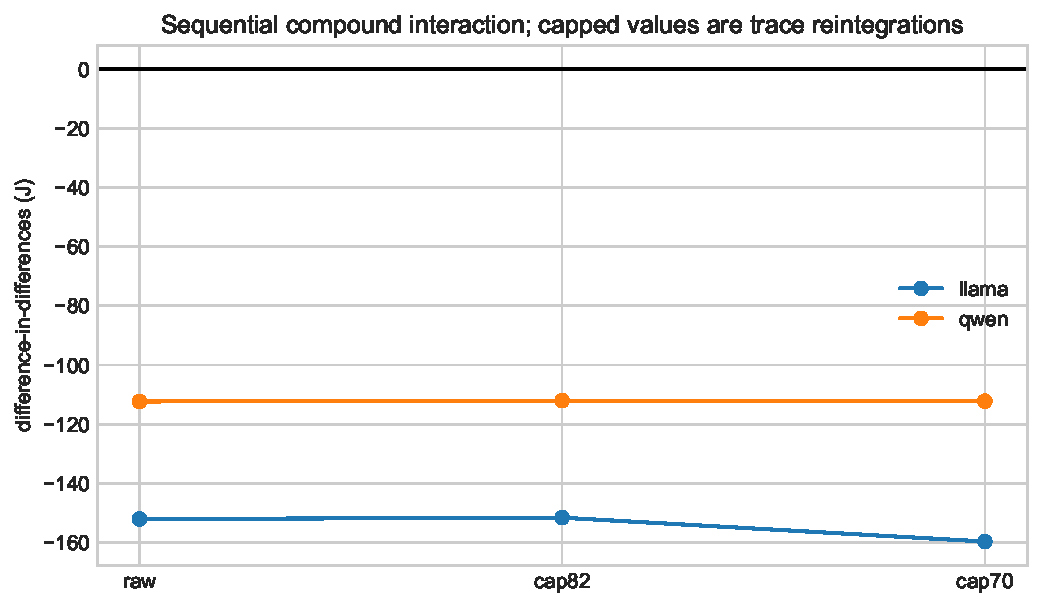
\includegraphics[width=\columnwidth]{figures/fig_interaction_by_power_regime.pdf}
\Description{A grouped bar chart shows negative eviction--TQ interaction values for Llama and Qwen under raw, 82-watt-capped, and 70-watt-capped power traces.}
\caption{Sequential compound interaction ($I$) for Llama (left, orange) and Qwen (right, blue) under raw, 82~W-capped, and 70~W-capped trace integration. Both values remain strictly negative, demonstrating that eviction consistently shields quantization overhead across power clipping regimes.}
\label{fig:interaction}
\end{figure}

As shown in Figure~\ref{fig:interaction}, this negative interaction held equally for Qwen ($I = -112.32$~J) and remained stable under artificial power trace capping.

\subsection{Llama: System Trade-Offs at 4096 Tokens}

The empirical trade-offs between decode throughput, energy consumption, peak VRAM, and active KV cache volume are detailed in Table~\ref{tab:llama-all} (and plotted in Appendix~\ref{app:context-scaling}, Figure~\ref{fig:tradeoffs}). In throughput versus energy, C2 forms the empirical efficiency boundary, achieving the highest throughput (20.34~tok/s) and lowest energy (529.30~J). In memory allocation, C3 incurs both the largest live cache (697~MiB) and highest peak VRAM (9468~MiB), whereas C2 minimizes both footprint metrics (119~MiB cache, 8500~MiB peak VRAM).

\subsection{Llama: Hard-Retrieval Quality}

Table~\ref{tab:llama-quality} reports retrieval accuracy on the frozen 60-scenario benchmark.

\begin{table}[htbp]
\caption{Llama Hard-Retrieval Accuracy at 4096 Tokens (60 Scenarios)}
\label{tab:llama-quality}
\centering\small
\begin{tabular}{lrrl}
\toprule
\textbf{Config} & \textbf{Pass/60} & \textbf{Rate} & \textbf{Wilson 95\% CI} \\
\midrule
C0 (FP16)     & 47/60 & 0.783 & $[0.664,\ 0.869]$ \\
C1-W (AWQ)    & 38/60 & 0.633 & $[0.507,\ 0.744]$ \\
C2 (Evict)    & 37/60 & 0.617 & $[0.490,\ 0.729]$ \\
C3-Ref (TQ)   & 37/60 & 0.617 & $[0.490,\ 0.729]$ \\
C4-Ref (Both) & 37/60 & 0.617 & $[0.490,\ 0.729]$ \\
\bottomrule
\end{tabular}
\end{table}

\begingroup\raggedright
Uncompressed FP16 (C0) achieved the highest retrieval accuracy (47/60 vs.\ 38/60 for AWQ). Among the compressed variants, C2, C3-Ref, and C4-Ref each differed from the AWQ baseline (C1-W) by only one scenario (37/60 vs.\ 38/60). Analysis of failure cases showed that incorrect outputs were primarily distractor key confusions rather than missing responses or formatting errors.
\par\endgroup

Table~\ref{tab:depth} details performance across needle insertion depths. All configurations achieved highest accuracy at 10\% depth (beginning of the prompt) and lower accuracy at 50\% and 90\% depths.

\begin{table}[htbp]
\caption{Llama Retrieval Accuracy by Insertion Depth}
\label{tab:depth}
\centering\small
\begin{tabular}{lrrr}
\toprule
\textbf{Config} & \textbf{10\%} & \textbf{50\%} & \textbf{90\%} \\
\midrule
C0     & 19/20 & 13/20 & 15/20 \\
C1-W   & 18/20 & 10/20 & 10/20 \\
C2     & 18/20 & 10/20 &  9/20 \\
C3-Ref & 18/20 & 10/20 &  9/20 \\
C4-Ref & 17/20 & 10/20 & 10/20 \\
\bottomrule
\end{tabular}
\end{table}

\subsection{Pareto Frontier and Bootstrap Stability}

Table~\ref{tab:pareto3} presents the empirical three-objective Pareto frontier across total energy, hard-retrieval accuracy, and persistent KV cache footprint at 4096 tokens, evaluated over 2000 bootstrap resamples.

Figure~\ref{fig:pareto3obj} displays the multi-objective frontier. Marker area represents persistent KV cache volume, horizontal error bars denote energy standard deviation, vertical error bars denote Wilson 95\% confidence intervals for retrieval, and border thickness indicates bootstrap frontier-selection stability.

\begin{figure*}[htbp]
\centering
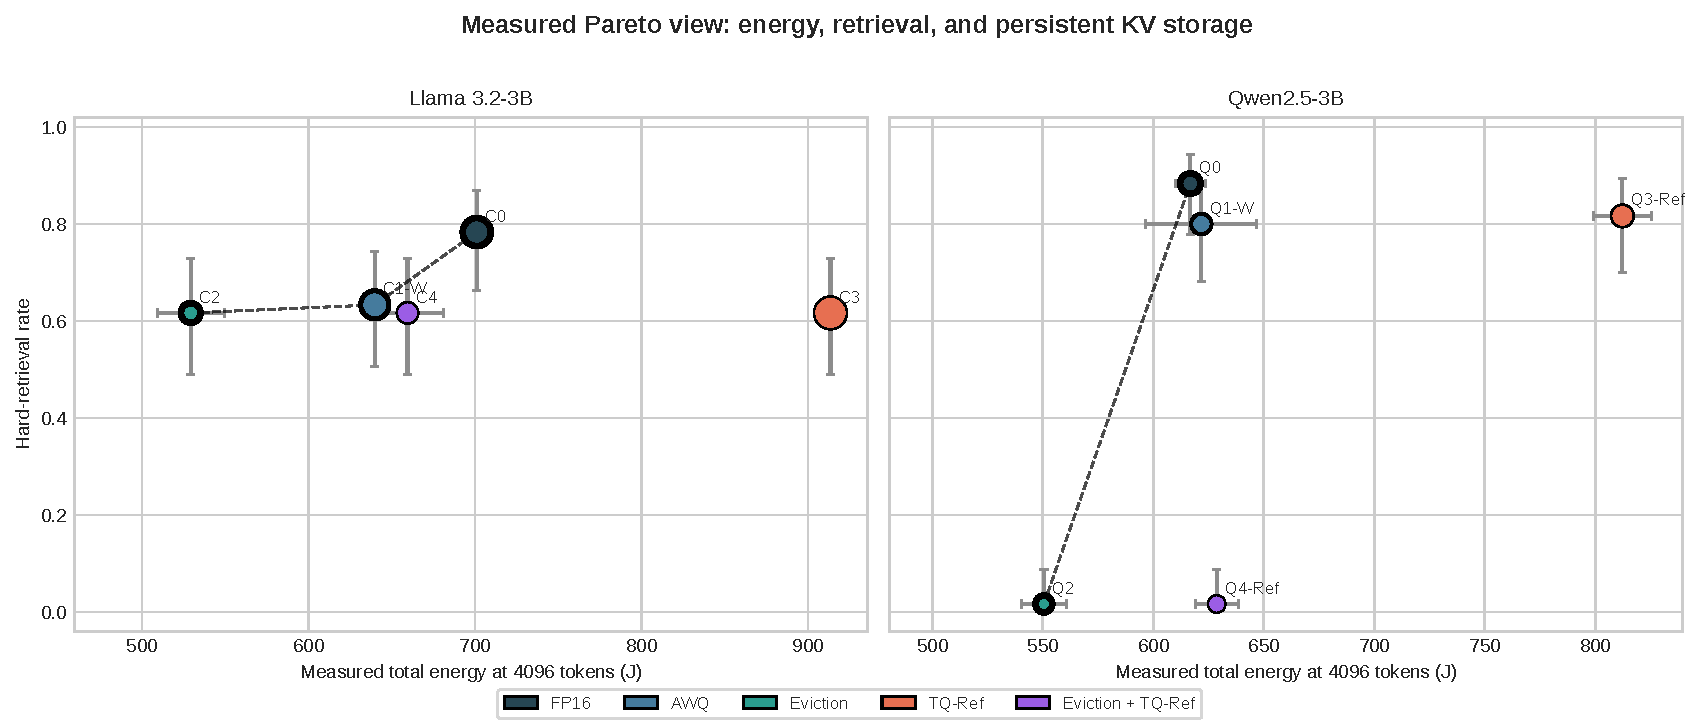
\includegraphics[width=\textwidth]{figures/fig08_measured_pareto_energy_quality_memory.pdf}
\Description{Two Pareto plots compare energy, retrieval quality, and persistent cache storage for Llama and Qwen at 4096 tokens.}
\caption{Empirical energy, quality, and memory Pareto frontier at 4096 tokens. Each marker denotes one configuration; marker area encodes persistent KV cache storage; horizontal bars show energy standard deviation; vertical bars show Wilson 95\% confidence intervals; border width represents bootstrap frontier-selection stability (2000 resamples). Left: Llama. Right: Qwen. Qwen exhibits complete separation between low-energy, zero-retrieval eviction (Q2) and high-energy, high-retrieval quantization (Q3-Ref).}
\label{fig:pareto3obj}
\end{figure*}

For Llama, C2 achieves the most favorable balance among measured points: lowest total energy (529.30~J), smallest persistent cache (119~MiB), highest throughput (20.34~tok/s), and retrieval accuracy within one scenario of baseline (37/60 vs.\ 38/60), with 100\% bootstrap selection stability. While C0 (100\%) and C1-W (63.0\%) also qualify as Pareto-optimal due to higher retrieval fidelity, C3 (0\%) and C4 (0.6\%) are dominated. Crucially, C2 strictly outperforms C4 across every operational dimension (19.7\% lower energy, 62.3\% higher throughput, 36.4\% smaller cache) with identical accuracy (37/60), demonstrating that naive disjoint sequential stacking is an empirical anti-pattern on real silicon compared to single-stage eviction.

For Qwen, the Pareto front divides into disjoint extremes: uncompressed Q0 provides the highest retrieval accuracy (0.883, 97.2\% bootstrap frequency), while eviction (Q2) achieves 100\% selection on energy and memory metrics but violates basic utility constraints with 1/60 retrieval. Q3-Ref was selected in only 3.8\% of resamples because its energy penalty outweighed its marginal retrieval gain over Q1-W.

Bootstrap frontier frequency quantifies resampling stability rather than a population probability of optimality. Importantly, Pareto membership alone is not a deployment recommendation; an explicit minimum quality threshold is necessary to filter out non-viable configurations like Q2.

\begin{table}[htbp]
\caption{Three-Objective Pareto Frontier at 4096 Tokens (2000 Bootstrap Resamples)}
\label{tab:pareto3}
\centering\small
\resizebox{\columnwidth}{!}{%
\begin{tabular}{@{}llrrrl@{}}
\toprule
\textbf{Model} & \textbf{Config} & \textbf{Energy (J)} & \textbf{Retrieval} & \textbf{Cache (MiB)} & \textbf{Boot.\%} \\
\midrule
Llama & C0     & 701.08 & 0.783 & 455 & 100.0\% \\
Llama & C1-W   & 639.86 & 0.633 & 455 &  63.0\% \\
Llama & C2     & 529.30 & 0.617 & 119 & 100.0\% \\
Llama & C3     & 913.48 & 0.617 & 697 &   0.0\% \\
Llama & C4     & 659.50 & 0.617 & 187 &   0.6\% \\
\midrule
Qwen  & Q0     & 616.78 & 0.883 & 146 &  97.2\% \\
Qwen  & Q1-W   & 621.75 & 0.800 & 146 &  36.0\% \\
Qwen  & Q2     & 550.48 & 0.017 &  38 & 100.0\% \\
Qwen  & Q3-Ref & 812.28 & 0.817 & 224 &   3.8\% \\
Qwen  & Q4-Ref & 628.69 & 0.017 &  60 &   0.0\% \\
\bottomrule
\end{tabular}}
\begin{minipage}{\columnwidth}\vspace{2pt}\footnotesize
Boot.\%: percentage of 2000 bootstrap resamples in which the configuration was
selected as a Pareto-optimal point. Higher values indicate greater frontier stability.
\end{minipage}
\end{table}

\subsection{Power Trace Robustness and Sensitivity}
\label{sec:robustness}

Raw NVML power traces recorded occasional transient spikes exceeding the nominal 70~W threshold, including isolated samples above 100~W and a maximum reading of 124.5~W on Llama (116.1~W on Qwen). To evaluate sensitivity to measurement artifacts, we reintegrated all 100 Llama power traces under an 82~W cap and a strict 70~W cap. Energy rank orderings ($\text{C2} < \text{C1} < \text{C4} < \text{C0} < \text{C3}$) and all five registered statistical significance decisions remained completely invariant across clipping thresholds (documented and plotted in Appendix~\ref{app:power-samples}, Figure~\ref{fig:power-cap} and Figure~\ref{fig:power-samples}).

\subsection{Sensitivity to Budget and Bit Width}

Sensitivity sweeps on Llama at 4096 tokens (plotted in Appendix~\ref{app:benchmark-pilots}, Figure~\ref{fig:sensitivity}) confirm that expanding the retained token budget slightly increases energy without altering retrieval accuracy on standard tasks, while higher nominal quantization precision improves retrieval fidelity without altering physical energy due to 8-bit container storage.

\subsection{Qwen: Energy Measurements}
\label{sec:qwen-energy}

Table~\ref{tab:qwen-all} summarizes Qwen2.5-3B energy consumption across context lengths. Unlike Llama, AWQ (Q1-W) did not yield energy savings relative to uncompressed FP16 (Q0) at any context length. At 4096 tokens, Q0 averaged 616.78~J compared to 621.75~J for Q1-W.

\begin{table}[htbp]
\caption{Qwen Energy (J, mean $\pm$ SD) Across Contexts}
\label{tab:qwen-all}
\centering\small
\resizebox{\columnwidth}{!}{%
\begin{tabular}{@{}lrrrrr@{}}
\toprule
\textbf{Context} & \textbf{Q0} & \textbf{Q1-W} & \textbf{Q2} & \textbf{Q3-Ref} & \textbf{Q4-Ref} \\
\midrule
1024 & $258.6\!\pm\!27.4$ & $293.4\!\pm\!21.6$ & $272.0\!\pm\!13.9$ & $358.6\!\pm\!9.6$  & $343.0\!\pm\!14.1$ \\
2048 & $334.2\!\pm\!17.5$ & $398.5\!\pm\!12.5$ & $342.6\!\pm\!10.3$ & $540.9\!\pm\!14.1$ & $435.2\!\pm\!20.0$ \\
4096 & $616.8\!\pm\!6.8$  & $621.8\!\pm\!25.1$ & $550.5\!\pm\!10.1$ & $812.3\!\pm\!13.1$ & $628.7\!\pm\!9.8$  \\
\bottomrule
\end{tabular}}
\end{table}

Eviction (Q2) required the lowest energy across all context lengths. At 4096 tokens, Q2 consumed 71.27~J less energy than Q1-W (an 11.5\% reduction), though the difference fell short of statistical significance after Holm correction ($p = 0.0656$). However, this energy reduction is accompanied by severe retrieval degradation (Section~\ref{sec:qwen-quality}).

\subsection{Qwen: Hard-Retrieval Quality}
\label{sec:qwen-quality}

Table~\ref{tab:qwen-quality} reports hard-retrieval accuracy for Qwen2.5-3B.

\begin{table}[htbp]
\caption{Qwen Hard-Retrieval Accuracy at 4096 Tokens (60 Scenarios)}
\label{tab:qwen-quality}
\centering\small
\begin{tabular}{lrrl}
\toprule
\textbf{Config} & \textbf{Pass/60} & \textbf{Rate} & \textbf{Wilson 95\% CI} \\
\midrule
Q0 (FP16)     & 53/60 & 0.883 & $[0.778,\ 0.942]$ \\
Q1-W (AWQ)    & 48/60 & 0.800 & $[0.682,\ 0.882]$ \\
Q2 (Evict)    & 1/60  & 0.017 & $[0.003,\ 0.089]$ \\
Q3-Ref (TQ)   & 49/60 & 0.817 & $[0.701,\ 0.894]$ \\
Q4-Ref (Both) & 1/60  & 0.017 & $[0.003,\ 0.089]$ \\
\bottomrule
\end{tabular}
\end{table}

Eviction (Q2) reduced retrieval accuracy to 1/60 across all document depths (0/20 at 10\%, 0/20 at 50\%, 1/20 at 90\%). Paired comparison against Q1-W showed 47 performance losses and 0 gains (exact McNemar $p = 1.71 \times 10^{-13}$). Compound compression (Q4-Ref) also collapsed to 1/60, inheriting the failure of the eviction stage.

Conversely, TurboQuant reference (Q3-Ref) maintained retrieval accuracy (49/60), closely matching Q1-W (48/60), while increasing total energy consumption by 190.53~J (30.6\%) to 812.28~J.

\subsection{Cross-Model Quality Contrast}

The cross-model eviction contrast $(\Delta_{\text{Qwen}} - \Delta_{\text{Llama}})$ was $-0.767$ (depth-stratified bootstrap 95\% CI: $[-0.867, -0.667]$): eviction degraded retrieval accuracy on Qwen by 76.7 percentage points more than on Llama. Comparative Wilson confidence intervals across all configurations and bit widths are plotted in Appendix~\ref{app:benchmark-pilots} (Figure~\ref{fig:wilson}). While this highlights substantial architecture sensitivity, our two-model comparison does not isolate whether the collapse stems from GQA head ratios, vocabulary tokenization, or layerwise budget allocation.

\subsection{Qwen Sensitivity Sweep}

Table~\ref{tab:qwen-sensitivity} summarizes the sensitivity results for Qwen. Expanding the average eviction budget by 50\% (from 1024 to 1536 retained tokens) recovered only 2/15 scenarios, indicating that failure is driven by token selection errors rather than insufficient capacity. In precision scaling, 2-bit quantization caused substantial retrieval loss (4/15), whereas 3-bit (11/15) and 4-bit (12/15) preserved accuracy. Measured energy showed minimal variation across bit widths because all variants execute within 8-bit containers in the reference package.

\begin{table}[htbp]
\caption{Qwen Sensitivity at 4096 Tokens (15 Common Scenarios)}
\label{tab:qwen-sensitivity}
\centering\small
\resizebox{\columnwidth}{!}{%
\begin{tabular}{@{}lrrl@{}}
\toprule
\textbf{Variant} & \textbf{Energy (J)} & \textbf{Retrieval} & \textbf{Wilson 95\% CI} \\
\midrule
\multicolumn{4}{l}{\textit{PyramidKV budget sweep}} \\
Q2-B512  & $515.2 \pm 8.9$  & 0/15 & $[0.000,\ 0.218]$ \\
Q2-B1024 & $550.5 \pm 10.1$ & 1/15 & $[0.003,\ 0.234]$ \\
Q2-B1536 & $590.6 \pm 13.2$ & 2/15 & $[0.026,\ 0.320]$ \\
\midrule
\multicolumn{4}{l}{\textit{TurboQuant bit-width sweep}} \\
Q3-Ref-TQ2 & $808.9 \pm 34.0$ & 4/15  & $[0.109,\ 0.520]$ \\
Q3-Ref-TQ3 & $791.3 \pm 19.6$ & 11/15 & $[0.480,\ 0.891]$ \\
Q3-Ref-TQ4 & $812.3 \pm 13.1$ & 12/15 & $[0.548,\ 0.930]$ \\
\bottomrule
\end{tabular}}
\end{table}

\subsection{Memory Footprint and Realization Analysis}

Table~\ref{tab:storage} provides exact memory quantities during decoding at 4096 tokens, comparing the unquantized baseline, the realized reference implementation, and theoretical ideal packed quantization (analyzed in detail in Appendix~\ref{app:ideal}, Figure~\ref{fig:storage} and Figure~\ref{fig:tq_realization}).

\begin{table}[htbp]
\caption{Decode Storage at 4096 Tokens: Measured vs.\ Ideal (MiB)}
\label{tab:storage}
\centering\small
\resizebox{\columnwidth}{!}{%
\begin{tabular}{@{}lrrrr@{}}
\toprule
\textbf{Path} & \textbf{Non-TQ base} & \textbf{Realized TQ-Ref} & \textbf{Ideal packed} & \textbf{Ideal/FP16} \\
\midrule
Llama TQ-only   & 455.00 & 696.50 & 131.14 & 28.8\% \\
Llama evict.+TQ & 119.00 & 187.25 &  41.89 & 35.2\% \\
Qwen TQ-only    & 146.25 & 223.88 &  42.15 & 28.8\% \\
Qwen evict.+TQ  &  38.25 &  60.19 &  13.46 & 35.2\% \\
\bottomrule
\end{tabular}}
\begin{minipage}{\columnwidth}\vspace{2pt}\footnotesize
Ideal values are theoretical estimates assuming packed indices at nominal bit
width, FP32 norms, 128-token FP16 residual, and fused reconstruction. No such
implementation was measured.
\end{minipage}
\end{table}


%% ════════════════════════════════════════════════════════════════
%%  6. DISCUSSION
%% ════════════════════════════════════════════════════════════════
\section{Discussion}

\subsection{Divergence Between Expectations and Empirical Findings}

Prior literature suggests that combining weight quantization, token eviction, and KV-cache compression should yield compounding reductions in energy and memory footprint while maintaining task performance. Table~\ref{tab:hypotheses} contrasts these initial expectations with our empirical measurements.

\begin{table}[htbp]
\caption{Initial Expectations versus Empirical Findings}
\label{tab:hypotheses}
\centering\small
\resizebox{\columnwidth}{!}{%
\begin{tabular}{@{}>{\raggedright\arraybackslash}p{0.44\columnwidth}>{\raggedright\arraybackslash}p{0.52\columnwidth}@{}}
\toprule
\textbf{Expected} & \textbf{Observed Finding} \\
\midrule
AWQ saves $\sim$3$\times$ energy & Saves $\sim$10\% at 4096 tokens; increases energy at 1024 tokens \\
TurboQuant reduces memory 15\% to 20\% & Realized TQ-Ref increased storage by over 50\% \\
Eviction preserves retrieval & Preserved on Llama (37/60); collapsed on Qwen (1/60) \\
Sequential compound minimizes all costs & C4 not significantly lower than C1; Q4 collapsed to 1/60 \\
\bottomrule
\end{tabular}}
\end{table}

This divergence shows that theoretical compression ratios do not automatically translate to physical energy savings when software packages retain uncompressed state or when pruning heuristics encounter sensitive attention layouts.

\subsection{Eviction Divergence and Architecture Sensitivity}

The contrasting retrieval outcomes under token eviction represent the largest disparity in our data. Several architectural and experimental differences between Llama~3.2-3B and Qwen2.5-3B account for this behavior:
\begin{itemize}
  \item \textbf{GQA Head Sharing:} Qwen uses an 8:1 query-to-KV head ratio (2 KV heads across 16 query heads), compared to Llama's 3:1 ratio (8 KV heads across 24 query heads). In an 8:1 configuration, evicting a single KV token entry simultaneously strips historical context from eight distinct query heads.
  \item \textbf{Tokenization Density:} Differences in vocabulary and chat template formatting alter token sequences, which can shift important information relative to layer attention windows.
  \item \textbf{Heuristic Portability:} Attention-based importance heuristics developed primarily on balanced GQA structures transfer poorly to aggressive head sharing.
\end{itemize}

Crucially, our empirical sensitivity sweep rules out simple hyperparameter capacity mismatch as the primary cause: expanding the average retained token budget by 50\% (from 1024 to 1536 tokens, Table~\ref{tab:qwen-sensitivity}) recovered only two additional scenarios (2/15 pass rate). This confirms that retrieval collapse is driven by structural token selection errors under 8:1 GQA rather than insufficient memory capacity.

Figure~\ref{fig:eviction_gqa} illustrates how GQA geometry amplifies the impact of token removal.

\begin{figure*}[htbp]
\centering
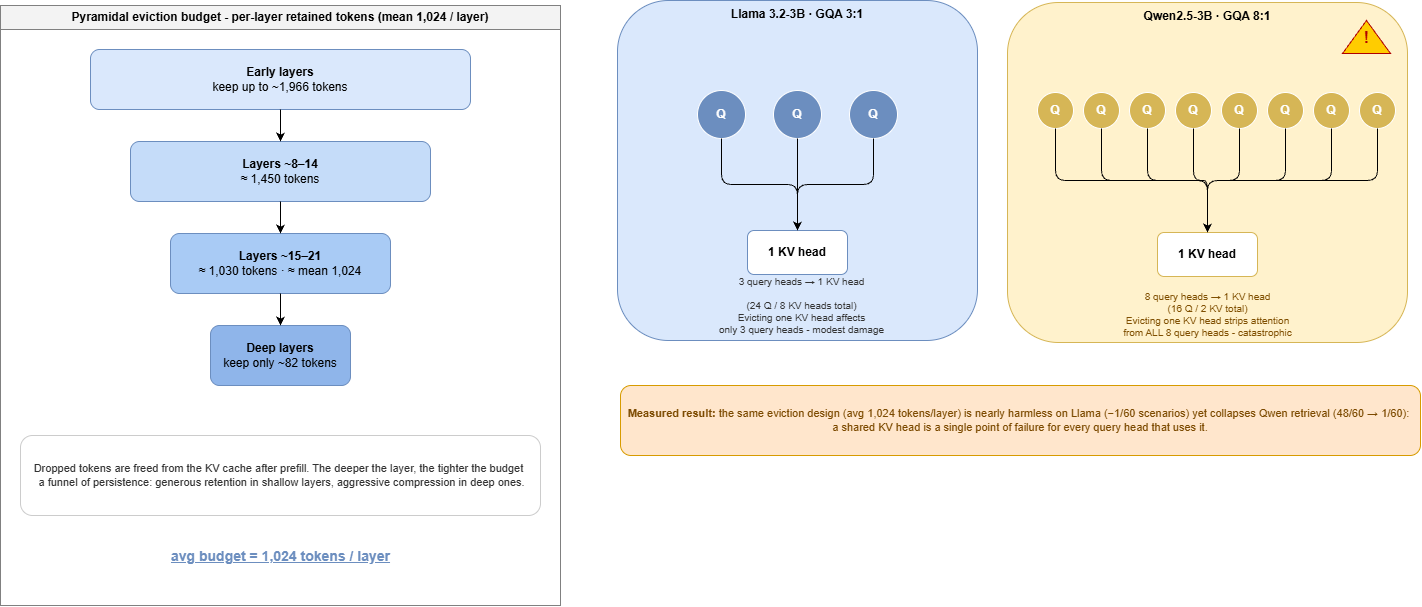
\includegraphics[width=\textwidth]{figures/eviction_graph.png}
\Description{A diagram compares pyramidal eviction budgets and grouped-query attention geometry: Llama shares each KV head with three query heads, while Qwen shares each KV head with eight query heads.}
\caption{Pyramidal token eviction budgets alongside Grouped-Query Attention (GQA) layouts. Under Qwen's 8:1 GQA ratio, removing a single KV token eliminates historical context across eight query heads simultaneously, contributing to severe retrieval degradation compared to Llama's 3:1 arrangement.}
\label{fig:eviction_gqa}
\end{figure*}

\subsection{Physical Execution versus Nominal Compression}

Our evaluation of TurboQuant reflects the numerical reference implementation rather than an optimized fused kernel. A production kernel that physically packs coordinate indices and fuses dequantization into the attention compute loop could approach the ideal memory targets in Table~\ref{tab:storage}. Reporting measured execution characteristics rather than theoretical projections provides an empirical baseline for future kernel development.

\subsection{Scope of Statistical Claims}

The registered experimental matrix establishes:
\begin{enumerate}
  \item Token eviction significantly reduces total energy consumption on Llama at 4096 tokens (Holm $p = 0.00549$).
  \item The TurboQuant reference package significantly increases total energy consumption across both models.
  \item Both models exhibit a statistically significant negative interaction ($I < 0, p < 0.01$), confirming that prior eviction reduces quantization workload.
  \item Token eviction severely degraded hard-retrieval performance on Qwen ($p = 1.71 \times 10^{-13}$).
  \item Energy rank orderings and significance decisions remained stable under 82~W and 70~W power trace clipping.
\end{enumerate}

Conversely, the data does not establish:
\begin{itemize}
  \item Strict energetic equivalence between C1-W and C4-Ref (the 95\% CI $[-60.28, 3.76]$~J spans zero but remains wide).
  \item That Qwen's retrieval failure was caused solely by GQA geometry to the exclusion of tokenization or attention patterns.
  \item That energy penalties in the reference implementation would persist in a custom fused CUDA kernel.
  \item That Llama's retrieval retention extends to context lengths beyond 4096 tokens or across open-ended reasoning tasks.
  \item That AWQ provides uniform energy savings across all sequence lengths.
\end{itemize}

\subsection{Bridging Sequential Stacking and Joint Optimization (RDKV and ThinKV)}
\label{sec:joint-opt}

Our empirical findings provide direct physical motivation for the emerging literature on joint rate-distortion compression. Theoretical frameworks such as \textbf{RDKV}~\cite{zhang_rdkv_2026} and \textbf{ThinKV}~\cite{ramachandran_thinkv_2026} propose dynamic, continuous bit allocation across tokens and layers, treating token eviction as an extreme case of zero-bit assignment within a rate-distortion objective.

While these frameworks demonstrate promising Pareto frontiers in algorithmic simulation, our hardware measurements expose the concrete failure modes of disjoint sequential pipelines that make joint optimization necessary on real devices. Specifically, our empirical Pareto frontier demonstrates that naive sequential stacking (C4) is strictly dominated by single-stage eviction (C2) on balanced architectures (Llama), while causing complete retrieval collapse (1/60) on aggressive head-sharing layouts (Qwen). Expanding Qwen's eviction budget by 50\% in our sensitivity sweep (Table~\ref{tab:qwen-sensitivity}) recovered only 2 out of 15 scenarios, confirming that discrete token selection errors drive the failure.

These physical silicon findings provide clear boundary conditions for RDKV and ThinKV: under aggressive GQA, retaining marginal tokens at low precision (such as 1 or 2 bits) is essential to preserve directional attention signals, whereas hard binary eviction discards them. Furthermore, our measurement of the sequential shielding effect ($I < 0$) proves that shrinking active cache volume prior to quantization yields genuine energy savings by decreasing DRAM read traffic. Consequently, our physical measurements provide both the baseline data and the practical justification for transitioning from disjoint sequential pipelines to hardware-fused joint rate-distortion engines on edge accelerators.


%% ════════════════════════════════════════════════════════════════
%%  7. THREATS TO VALIDITY
%% ════════════════════════════════════════════════════════════════
\section{Threats to Validity}

\subsection{Internal Validity}
All execution rows for a given model were collected within continuous runtime sessions on Google Colab. We recorded five independent energy measurement blocks per condition ($n=5$), providing sufficient statistical power to detect large effects while acknowledging wider confidence intervals for small differences. In Llama runs, compressed configurations (C2 to C4) were compared against stock AWQ (C1), where the custom wrapper introduced a minor baseline offset ($\approx 8.61$~J at 4096 tokens). On Qwen, the matched wrapper was applied uniformly across all configurations. Two in-session code repairs in Notebook~08 were retained inline, and all raw trace files were verified via SHA-256 integrity checksums rather than post-hoc reconstruction.

\subsection{Construct Validity}
Our quality evaluation focuses on structured key-value extraction across three controlled document positions. While this provides diagnostic headroom for memory compression, it does not assess multi-step reasoning, natural dialogue, summarization, or multilingual fluency. Furthermore, energy measurements reflect board-level GPU power sampled via NVML and do not capture host CPU dissipation, system memory power, or facility cooling overhead.

\subsection{External Validity}
Experiments were conducted on two open-weight 3B models on a single GPU architecture (NVIDIA T4). Because the two evaluated models differ in layer count (36 in Qwen vs.\ 28 in Llama), vocabulary tokenization (152k vs.\ 128k), and context scaling parameters alongside their GQA ratios (8:1 vs.\ 3:1), our findings identify GQA head sharing as the primary structural suspect but do not completely isolate it from other architectural confounds without synthetic ablation. Hardware execution on free-tier cloud environments introduces minor inter-session frequency variation, though within-session blocking mitigates confounding. Finally, teacher-forced 64-token decoding isolates compression mechanisms but does not capture dynamic sequence lengths in open-ended generation.

\subsection{Statistical Conclusion Validity}
Family-wise error rates were controlled using Holm sequential correction for energy contrasts and Bonferroni adjustments for McNemar tests. Wilson score intervals at $n=60$ span approximately $\pm 13$ percentage points, whereas $n=15$ sensitivity intervals span $\pm 20$ percentage points. Bootstrap Pareto frequencies quantify resampling selection stability under empirical variance rather than absolute probabilities of optimality.


%% ════════════════════════════════════════════════════════════════
%%  8. CONCLUSION
%% ════════════════════════════════════════════════════════════════
\section{Conclusion}

This empirical ablation study evaluated how 4-bit AWQ weight quantization, custom PyramidKV token eviction, and TurboQuant KV-cache quantization behave when stacked on two 3B-parameter small language models running on an NVIDIA T4 GPU. By continuously sampling physical board-level power at 10~Hz across context lengths up to 4096 tokens and measuring exact-match extraction on a calibrated 60-scenario hard-retrieval benchmark, our measurements reveal several clear operational trade-offs for edge inference.

Our primary finding is that compression efficiency depends on attention geometry and sequence length rather than nominal compression ratios alone. On Llama~3.2-3B (3:1 GQA), combining 4-bit AWQ with custom PyramidKV eviction (C2) formed the most effective configuration at 4096 tokens: delivering a statistically significant 101.95~J (16.15\%) total energy reduction, accelerating decode throughput by 47.7\% (from 13.77 to 20.34~tok/s), reducing active KV cache storage by 73.8\% (from 455~MiB to 119~MiB), and maintaining hard-retrieval accuracy within one scenario of baseline (37/60 vs.\ 38/60) with 100\% bootstrap selection stability. In contrast, applying the identical eviction policy to Qwen2.5-3B (8:1 GQA) caused hard-retrieval accuracy to collapse from 48/60 to 1/60, proving that spatial pruning heuristics cannot be assumed to transfer across grouped-query attention ratios without risking catastrophic context loss.

Our hardware measurements also expose practical systems effects that theoretical models overlook. We measured and verified a negative compound interaction ($I = -152.03$~J on Llama, $I = -112.32$~J on Qwen, both $p < 0.01$), showing that prior cache eviction acts as an energy shield by reducing the volume of data handled by downstream quantization routines. We also documented a substantial software-to-hardware realization gap in off-the-shelf quantization packages, where retaining uncompressed tensors alongside discrete indices in the TurboQuant reference path added 31\% to 45\% net energy overhead. All energy rankings and registered statistical decisions remained invariant under 82~W and 70~W power trace clipping, confirming measurement stability.

These physical silicon findings directly ground theoretical joint compression frameworks, such as RDKV and ThinKV, demonstrating why continuous rate-distortion bit allocation is necessary to prevent discrete token selection failures on aggressive GQA architectures. Future work should evaluate additional open-weight SLM architectures (such as Gemma, Mistral, and Phi-3) across varied GQA configurations, test adaptive eviction heuristics (e.g., SnapKV, ChunkKV, and Ada-KV) at native context limits (8K to 32K), build physically packed and fused custom CUDA/Triton kernels to close the realization gap, and directly benchmark joint rate-distortion optimizers against sequential baselines on edge silicon.


%% ════════════════════════════════════════════════════════════════
%%  9. REPRODUCIBILITY
%% ════════════════════════════════════════════════════════════════
\section{Reproducibility}
\label{sec:reproducibility}

All experiments were executed on an NVIDIA Tesla T4 GPU (Turing architecture, compute capability 7.5, 16~GB nominal VRAM with 14.56~GiB to 15.0~GiB addressable capacity across a 256-bit bus) hosted on Ubuntu Linux instances via Google Colab. Table~\ref{tab:reproducibility-specs} summarizes the hardware specifications, software runtime dependencies, model geometry, and experimental protocols.

\begin{table}[htbp]
\caption{Detailed Reproducibility Specifications and Environmental Parameters}
\label{tab:reproducibility-specs}
\centering\small
\resizebox{\columnwidth}{!}{%
\begin{tabular}{@{}ll@{}}
\toprule
\textbf{Parameter Category} & \textbf{Configuration / Specification} \\
\midrule
\multicolumn{2}{l}{\textit{Host and GPU Hardware}} \\
Host Environment & Linux x86\_64 (kernel 6.6.122+, glibc 2.35) on Google Colab \\
Host CPU / RAM & Intel Xeon CPU @ 2.00~GHz (2 vCPUs), 12.67~GB system memory \\
GPU Architecture & NVIDIA Tesla T4 (Turing, Compute Capability 7.5, 40 SMs) \\
VRAM Capacity & 16~GB nominal (14.56~GiB addressable, 256-bit bus) \\
Power Limits & 70.0~W default and enforced cap (NVML queried) \\
Power Telemetry & 10~Hz (100~ms interval) via \texttt{pynvml}, Riemann $\int P(t)\,dt$ \\
Robustness Caps & Raw trace, 82~W clipped, 70~W clipped \\
\midrule
\multicolumn{2}{l}{\textit{Software Runtime and Libraries}} \\
Deep Learning Stack & PyTorch 2.11.0+cu128, CUDA 12.8 \\
Model Framework & Hugging Face Transformers 5.12.1 (\texttt{ddb849ab...}) \\
Quantization Packages & \texttt{gptqmodel==7.1.0}, \texttt{accelerate==1.14.0} \\
KV Quantization & \texttt{turboquant==0.2.0} (source SHA-256: \texttt{7358e277...}) \\
Scientific Stack & Python 3.11/3.12, NumPy 2.2.6, SciPy 1.16.1/3, Pandas 2.2.2 \\
\midrule
\multicolumn{2}{l}{\textit{Model Checkpoints and Geometry}} \\
Llama 3.2-3B-Instruct & 28 layers, 24 Q / 8 KV heads (3:1 GQA), head dim 128 \\
Llama FP16 / AWQ Rev. & \texttt{006f5dcd...} / \texttt{272b3bde...} \\
Qwen2.5-3B-Instruct & 36 layers, 16 Q / 2 KV heads (8:1 GQA), head dim 128 \\
Qwen FP16 / AWQ Rev. & \texttt{aa8e7253...} / \texttt{3559b226...} \\
\midrule
\multicolumn{2}{l}{\textit{Compression and Eviction Configuration}} \\
Weight Quantization & AWQ GEMM INT4, group size 128, zero-point true \\
Token Eviction Policy & Custom PyramidKV (decay $\beta=20$, win 32, kernel 5) \\
Eviction Budget & Avg 1024 tokens (Llama: 28 layers; Qwen: 1966 to 82) \\
TurboQuant Reference & Coordinate uint8 indices, FP32 norms, 128-tok FP16 res. \\
Sequential Stacking & AWQ linear $\to$ attention eviction $\to$ TQ reference \\
\midrule
\multicolumn{2}{l}{\textit{Evaluation and Statistical Protocols}} \\
Quality Benchmark & Hard-retrieval NIAH UUID extraction (60 scenarios) \\
Context Lengths & 1024, 2048, 4096 tokens (64-token fixed greedy decode) \\
Energy Sample Blocks & $n=5$ independent measurement runs per condition \\
Statistical Inference & Paired $t$-test / Wilcoxon with Holm correction \\
Categorical Tests & Exact McNemar test with Bonferroni adjustment \\
Pareto Uncertainty & 2000 depth-stratified bootstrap resamples \\
\bottomrule
\end{tabular}}
\end{table}

\paragraph{Model Checkpoints and Packaging.}
All model weights were pinned by commit revision. The Llama FP16 baseline used
the Unsloth checkpoint~\cite{unsloth_2024}, while Llama AWQ used the
CasperHansen release~\cite{casperhansen_llama32_awq}. Qwen FP16 and AWQ revisions are recorded in
\path{research/experiment_registry.json}~\cite{qwen2024technical}.
Integrity manifests bind model revisions, software versions, datasets, experiment
fingerprints, row counts, trace checksums, and prompt-set SHA-256 hashes.

\paragraph{Notebooks and Diagnostics.}
The self-contained Jupyter notebooks are stored in
\path{experiments/track_a_failsafe_colab/}. Notebook~10 provides automated
hardware, NVML-limit, and library-build diagnostics that export JSON, LaTeX, and
Markdown artifacts. Notebook~09B performs derived CPU synthesis without Google
Drive dependencies.

\paragraph{Evidence Bundles.}
Five accepted measurement bundles and one visualization bundle are archived in
\path{evidence/accepted/}. Each includes raw NVML traces, quality shards, derived
analysis tables, and a cryptographic integrity manifest.

\paragraph{Independent Verifiability.}
External reviewers can independently verify:
(1) artifact manifest hashes against individual files;
(2) integrity manifests against claimed sample counts;
(3) energy integration via trapezoidal summation on raw NVML power series;
(4) retrieval success rates and Wilson score intervals from shard outputs;
(5) hypothesis test statistics from summary datasets; and
(6) analytical KV memory projections from model architectural specifications.

\paragraph{Re-Execution Boundary.}
Exact hardware scheduling and transient GPU frequencies vary across cloud instances. The Qwen full reference run (Notebook~08) incorporates two inline software repairs whose source code is SHA-256 bound in the registry.

%% ════════════════════════════════════════════════════════════════
%%  GENERATIVE AI USAGE STATEMENT
%% ════════════════════════════════════════════════════════════════
\section*{Generative AI Usage Statement}

Generative AI tooling was utilized in two capacities during the preparation of this manuscript: assisting in drafting initial boilerplate code for experiment orchestration and figure plotting, and aiding in bibliographic search and reference matching. All AI-assisted suggestions, numerical outputs, and citations were independently verified against source papers and experimental logs. The conceptual formulation, experimental designs, empirical analyses, and conclusions are the sole work of the authors.

%% ════════════════════════════════════════════════════════════════
%%  REFERENCES
%% ════════════════════════════════════════════════════════════════
%% Print all BibTeX entries, including uncited background references.
\nocite{*}
\bibliographystyle{ACM-Reference-Format}
\begingroup
\sloppy
\hbadness=10000
\bibliography{references}
\endgroup

%% ════════════════════════════════════════════════════════════════
%%  APPENDICES
%% ════════════════════════════════════════════════════════════════
\clearpage  %% flush all pending main-body floats before appendix
\appendix

\section{Ideal Packed/Fused TQ Analysis \& Storage Realization}
\label{app:ideal}

This appendix presents the storage realization analysis and mathematical ideal-layout decomposition from Notebook~09. All ideal figures quoted are theoretical estimates and not experimental measurements. No numerical ideal energy, latency, throughput, or peak-VRAM value is claimed.

\begin{figure*}[htbp]
\centering
\begin{subfigure}{0.48\textwidth}
\centering
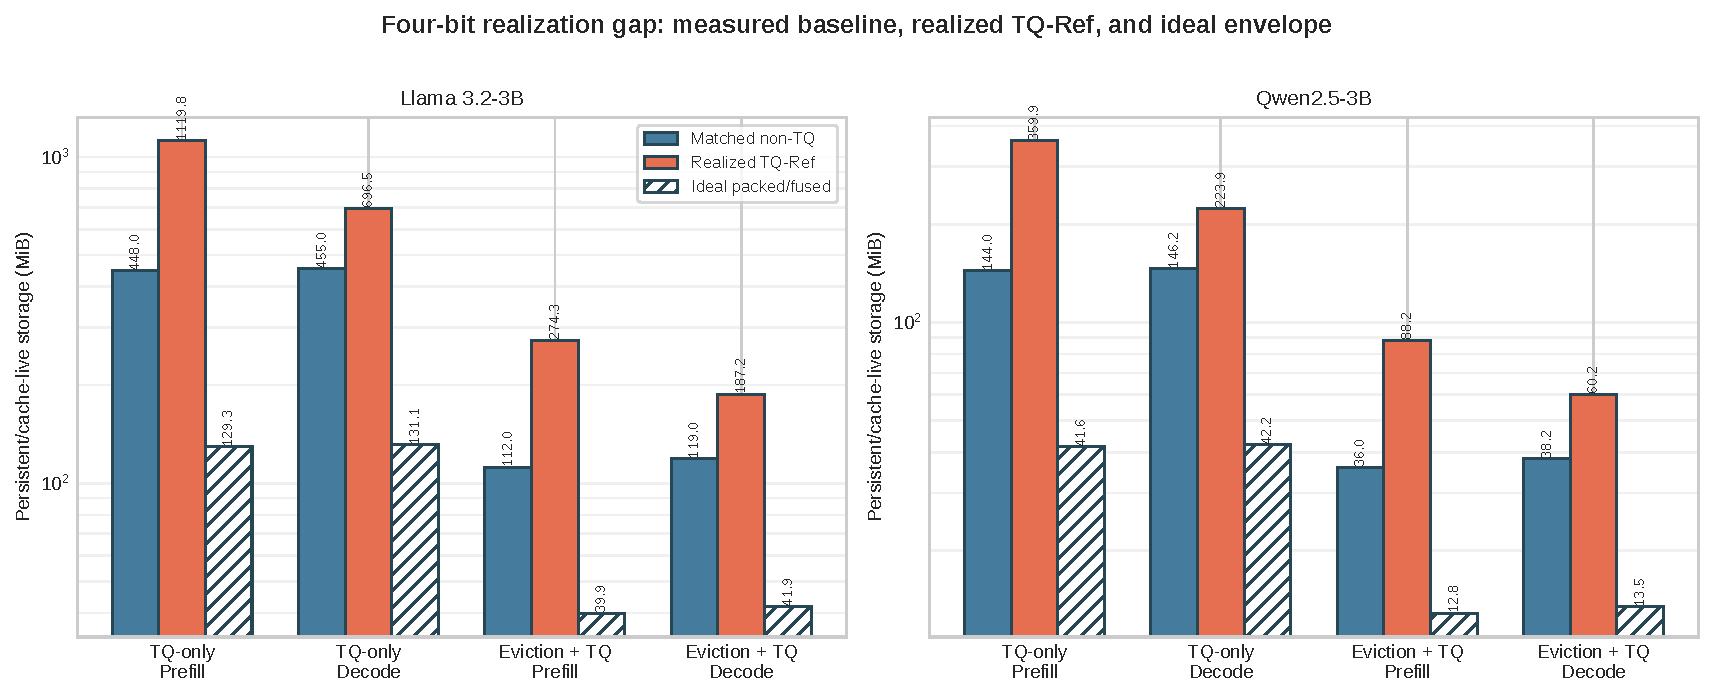
\includegraphics[width=\textwidth]{figures/fig04_storage_realization_gap.pdf}
\caption{Persistent KV cache footprint comparing baseline, realized TQ-Ref, and ideal packed layout (log scale).}
\label{fig:storage}
\end{subfigure}\hfill
\begin{subfigure}{0.48\textwidth}
\centering
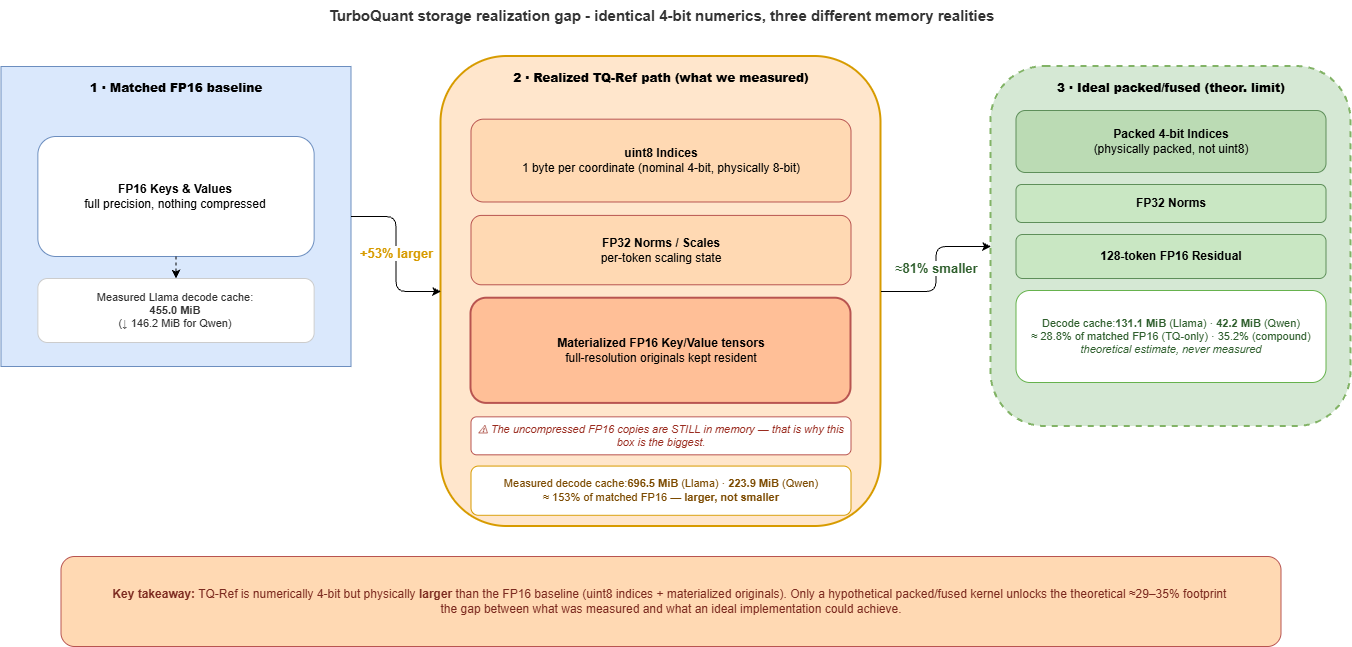
\includegraphics[width=\textwidth]{figures/turboquant_realization.png}
\caption{TQ-Ref retains FP16 KV tensors alongside \texttt{uint8} indices, unlike an ideal packed and fused layout.}
\label{fig:tq_realization}
\end{subfigure}

\vspace{3pt}
\begin{subfigure}[t]{0.64\textwidth}
\centering
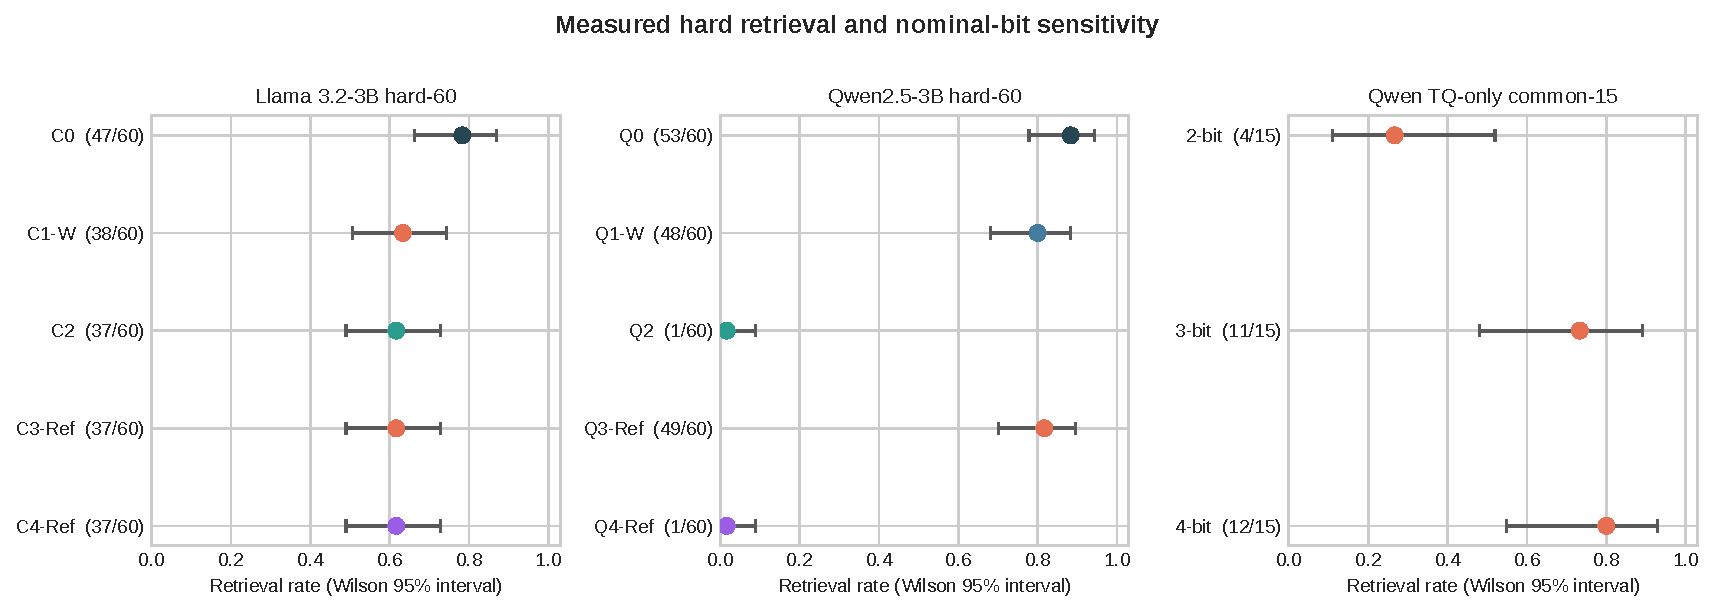
\includegraphics[width=\textwidth]{figures/fig03_retrieval_wilson.pdf}
\caption{Retrieval accuracy with Wilson 95\% confidence intervals at 4096 tokens.}
\label{fig:wilson}
\end{subfigure}\hfill
\begin{subfigure}[t]{0.32\textwidth}
\centering
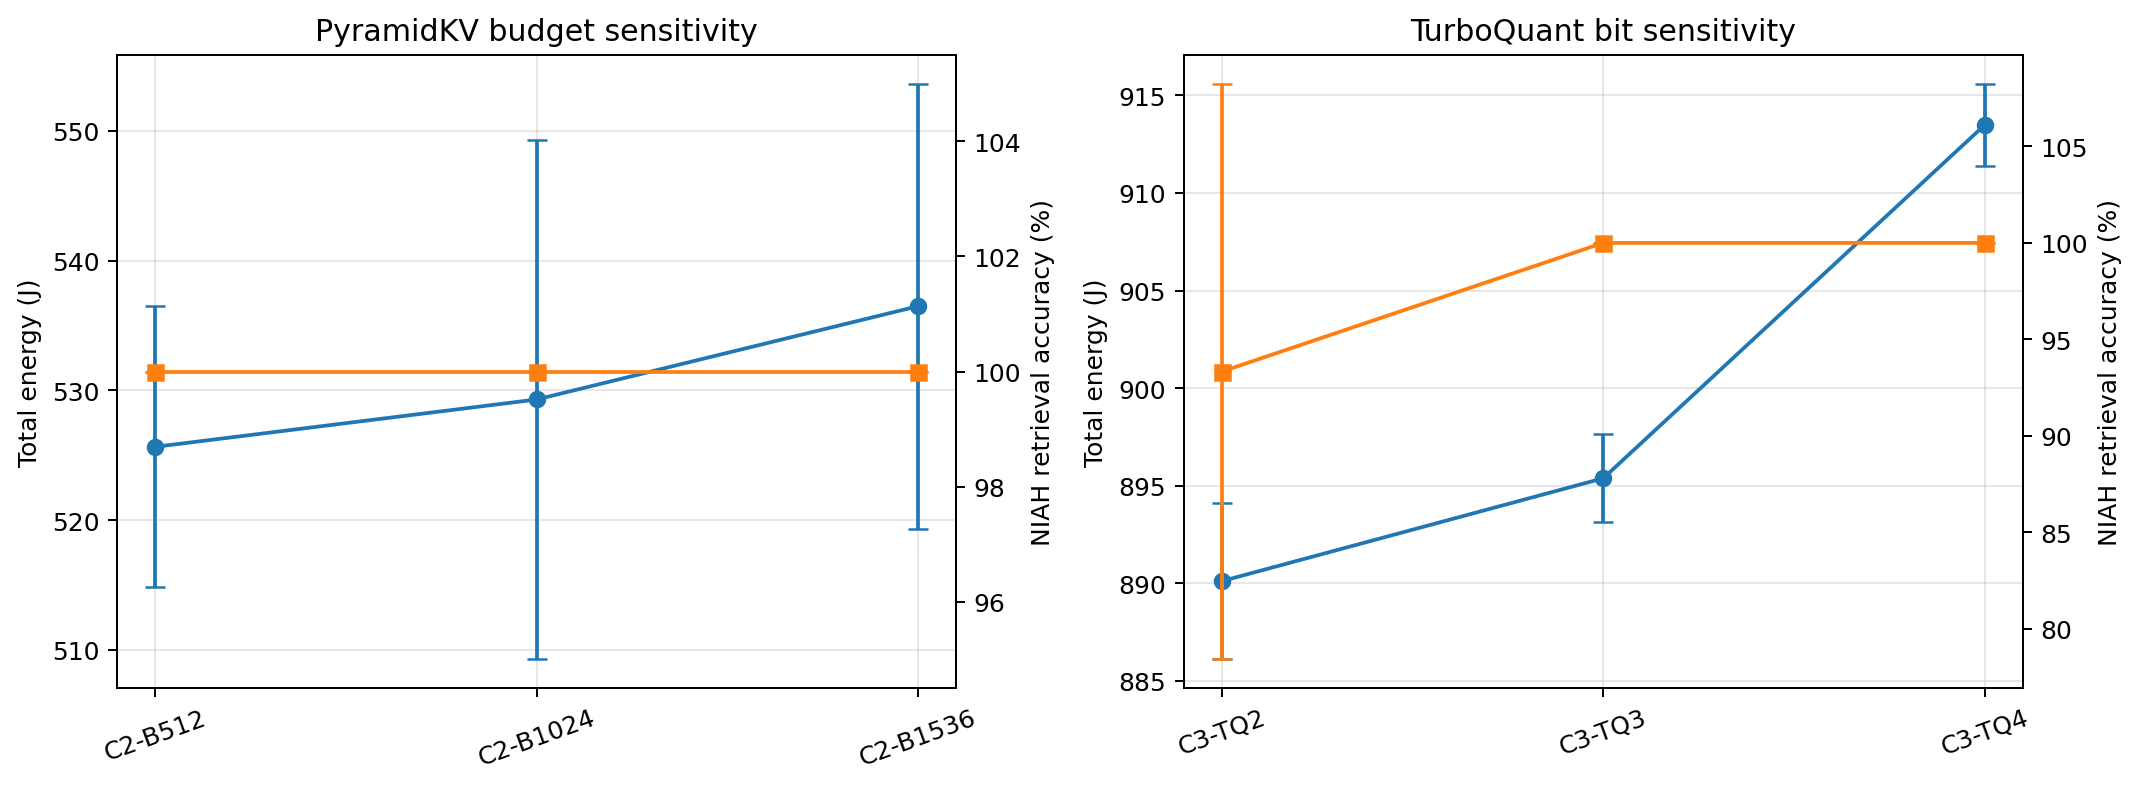
\includegraphics[width=\textwidth]{figures/v5_final_sensitivity_4096.png}
\caption{Llama sensitivity to eviction budget and quantization precision.}
\label{fig:sensitivity}
\end{subfigure}
\Description{Supplementary storage and retrieval diagnostics: realized versus ideal TurboQuant storage, tensor retention, retrieval confidence intervals, and sensitivity sweeps.}
\caption{Storage realization and retrieval diagnostics. Panels (a) and (b) show the TurboQuant storage realization gap; panels (c) and (d) show retrieval confidence intervals and Llama sensitivity analyses.}
\end{figure*}

\subsection{Ideal Storage Decomposition}

Figure~\ref{fig:ideal-components} illustrates how the four components of ideal storage (packed indices, FP32 norms, FP16 residual, and metadata) scale with bit width. Packed indices grow with bit width, while norms and residual remain fixed for a given retained-token structure. The normalized ratios are identical across Llama and Qwen because the model is geometry-normalized, which does not assert equal absolute byte counts.

If a future implementation packs indices at the nominal bit width and eliminates persistent materialized K/V tensors, decode storage ranges from $\approx$16.7\% of FP16 at 2~bits to $\approx$28.8\% at 4~bits for TQ-only, or $\approx$24.2\% to $\approx$35.2\% with prior eviction. The compound ratios are higher than TQ-only because the fixed 128-token residual constitutes a larger proportion of a smaller evicted cache.

\subsection{Modeled Phase Byte Demand}

Figure~\ref{fig:phase-demand} models logical compulsory dataflow rather than exact DRAM transactions. Prefill cannot claim compressed attention reads because full-prompt attention occurs before eviction or quantized persistence. Packing introduces a conversion read and compressed writes. Decode then repeatedly reads the growing cache, where an efficient fused implementation can potentially avoid materialized reconstruction writes.

\subsection{Symbolic Break-Even Boundary}

The ideal energy model is:
\begin{equation}
E_\text{ideal} = E_\text{baseline} - \epsilon_\text{mem} \cdot \Delta_D + O_\text{net}
\end{equation}
where $\epsilon_\text{mem}$ is the effective energy per avoided modeled byte and $O_\text{net}$ encompasses rotation, packing compute, reconstruction compute, and control overhead. When $\Delta_D > 0$ (representing decode savings), achieving a net energy reduction requires $O_\text{net} < \epsilon_\text{mem} \cdot \Delta_D$.

Figure~\ref{fig:break-even} shows the maximum allowable ratio $O_\text{net}/\epsilon_\text{mem}$ for each path. The boundary is widest for non-evicted 2-bit paths and smallest for compound 4-bit paths. Because no finite values are assigned to either unknown, this serves as a conditional reference rather than an empirical energy forecast.

\begin{figure*}[!t]
\centering
\begin{subfigure}{0.76\textwidth}
\centering
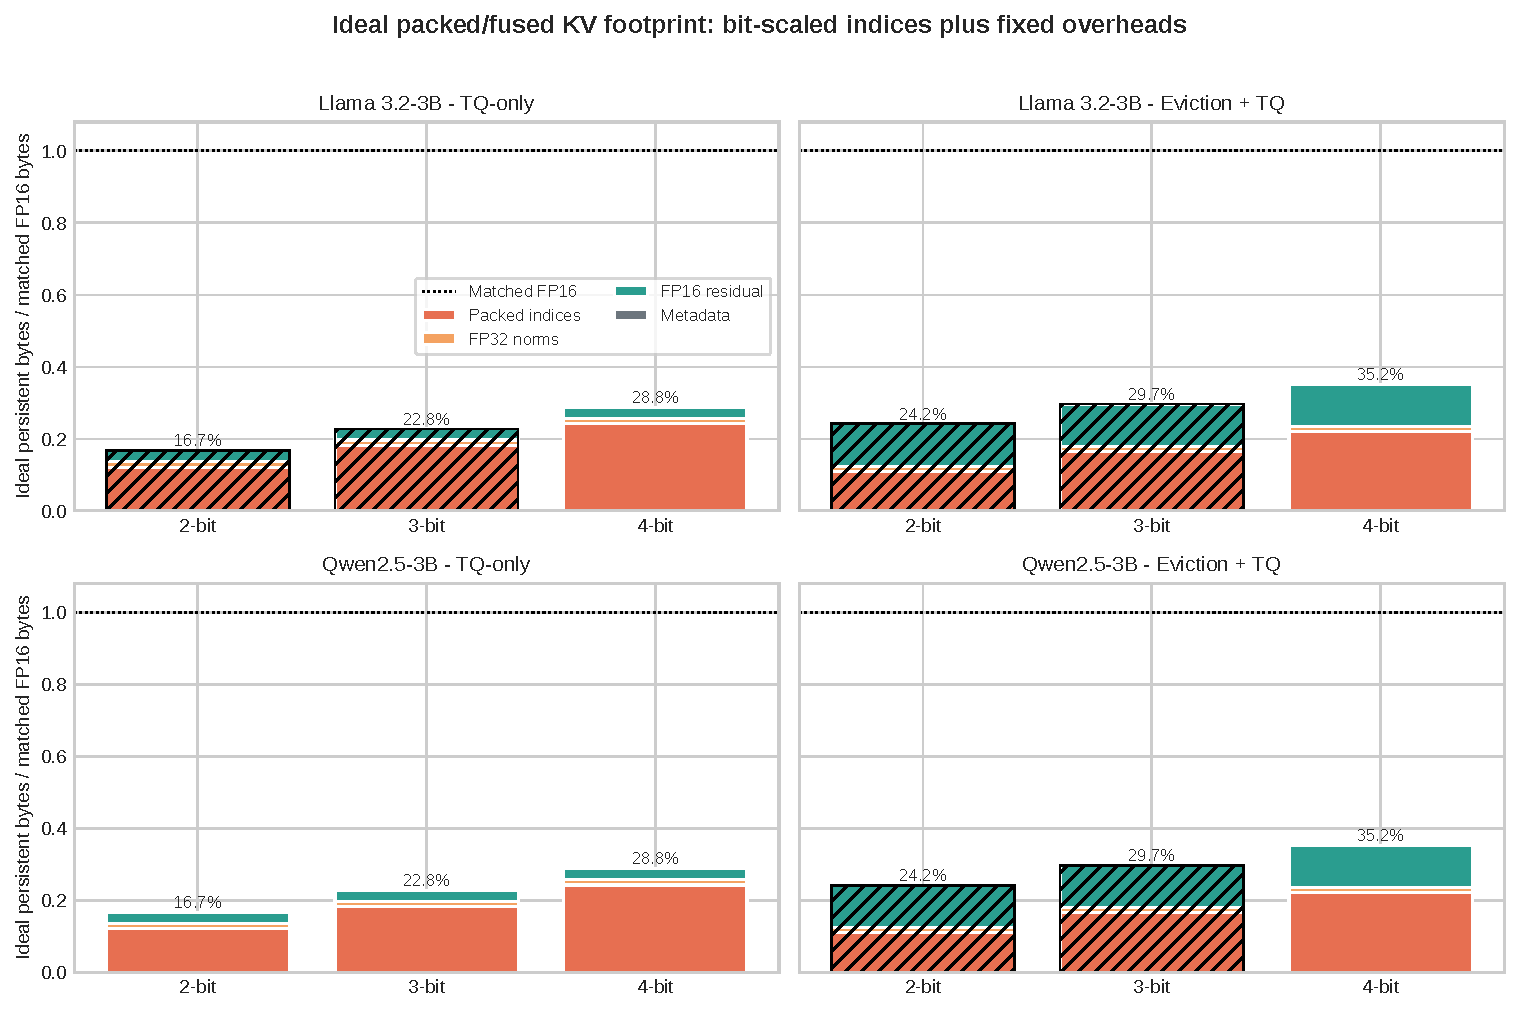
\includegraphics[width=\textwidth]{figures/fig05_ideal_packed_components.pdf}
\caption{Ideal packed/fused KV footprint, decomposed into packed indices, FP32 norms, FP16 residual, and metadata.}
\label{fig:ideal-components}
\end{subfigure}

\vspace{3pt}
\begin{subfigure}[t]{0.48\textwidth}
\centering
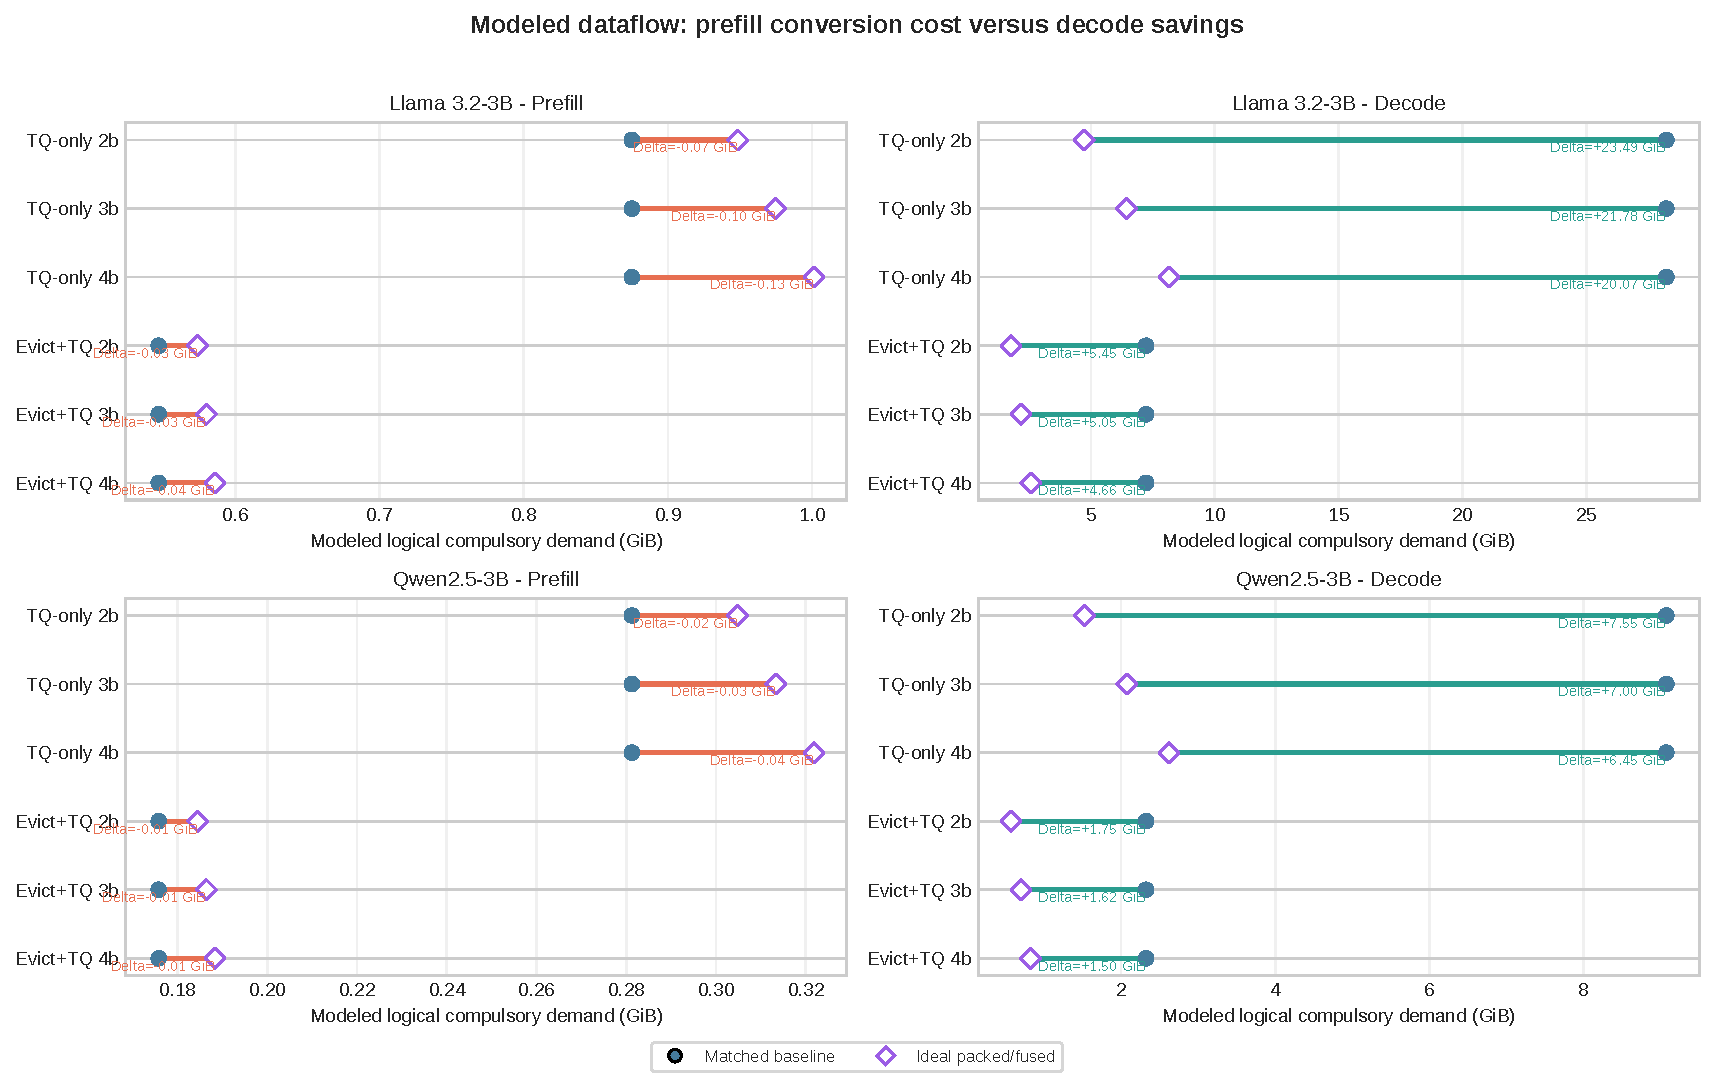
\includegraphics[width=\textwidth]{figures/fig06_modeled_phase_byte_demand.pdf}
\caption{Modeled compulsory dataflow for baseline and ideal packed/fused paths during prefill and decode.}
\label{fig:phase-demand}
\end{subfigure}\hfill
\begin{subfigure}[t]{0.48\textwidth}
\centering
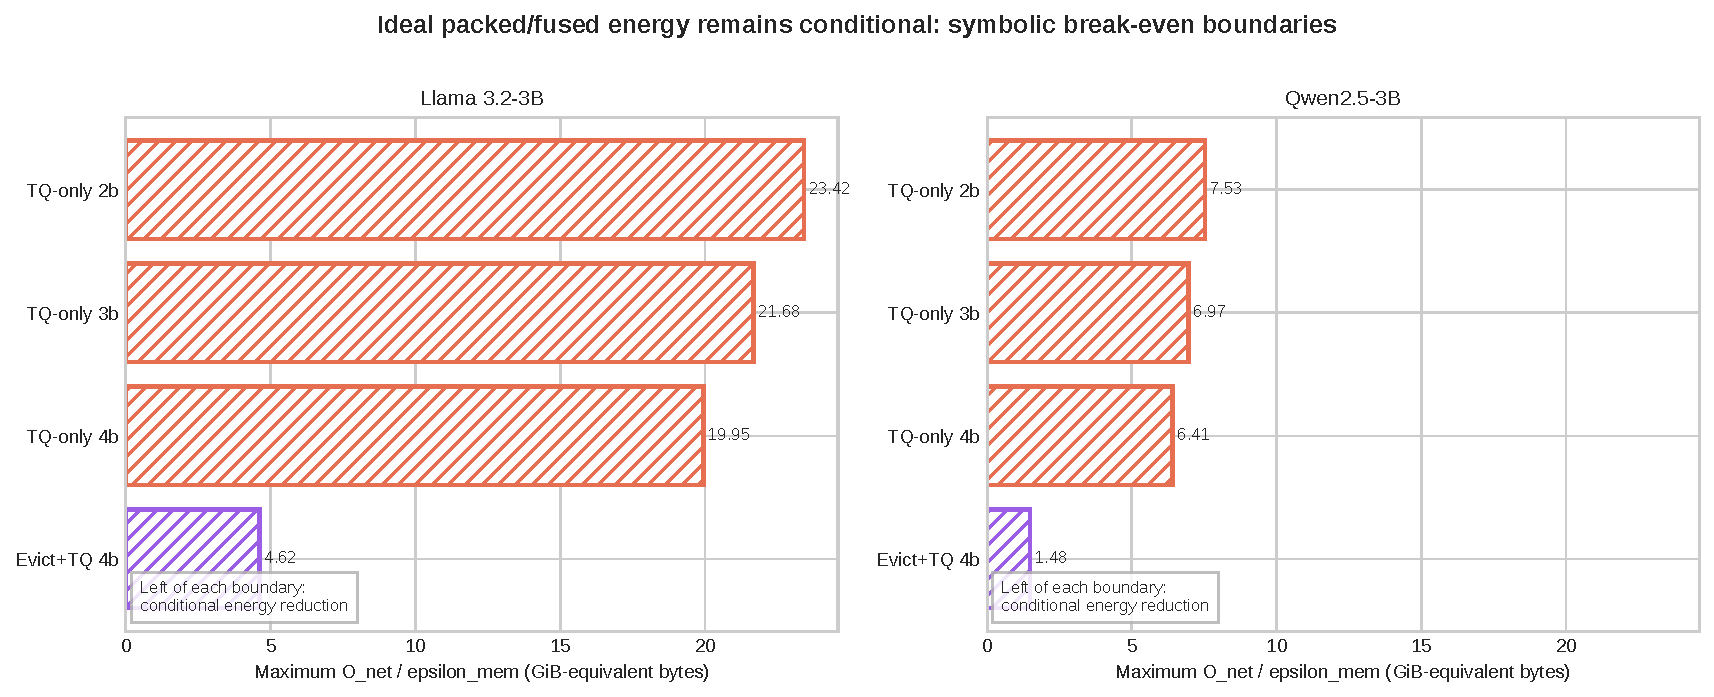
\includegraphics[width=\textwidth]{figures/fig07_symbolic_energy_break_even.pdf}
\caption{Symbolic break-even bounds for the ideal compressed KV-cache paths.}
\label{fig:break-even}
\end{subfigure}
\Description{Three appendix diagrams summarize ideal KV-cache compression: a footprint decomposition, modeled dataflow, and symbolic energy break-even bounds.}
\caption{Compact overview of the ideal packed/fused TurboQuant analysis. All values are theoretical estimates, not experimental measurements.}
\end{figure*}

%% ════════════════════════════════════════════════════════════════
%%  APPENDIX B: CONTEXT SCALING & PHASE OVERHEAD BREAKDOWN
%% ════════════════════════════════════════════════════════════════
\section{Context Scaling, Trade-Offs, and Phase Overhead}
\label{app:context-scaling}

This appendix provides extended visual characterizations of context scaling trends, phase-decomposed energy overheads, and two-dimensional system trade-offs.

\begin{figure*}[htbp]
\centering
\begin{subfigure}{0.48\textwidth}
\centering
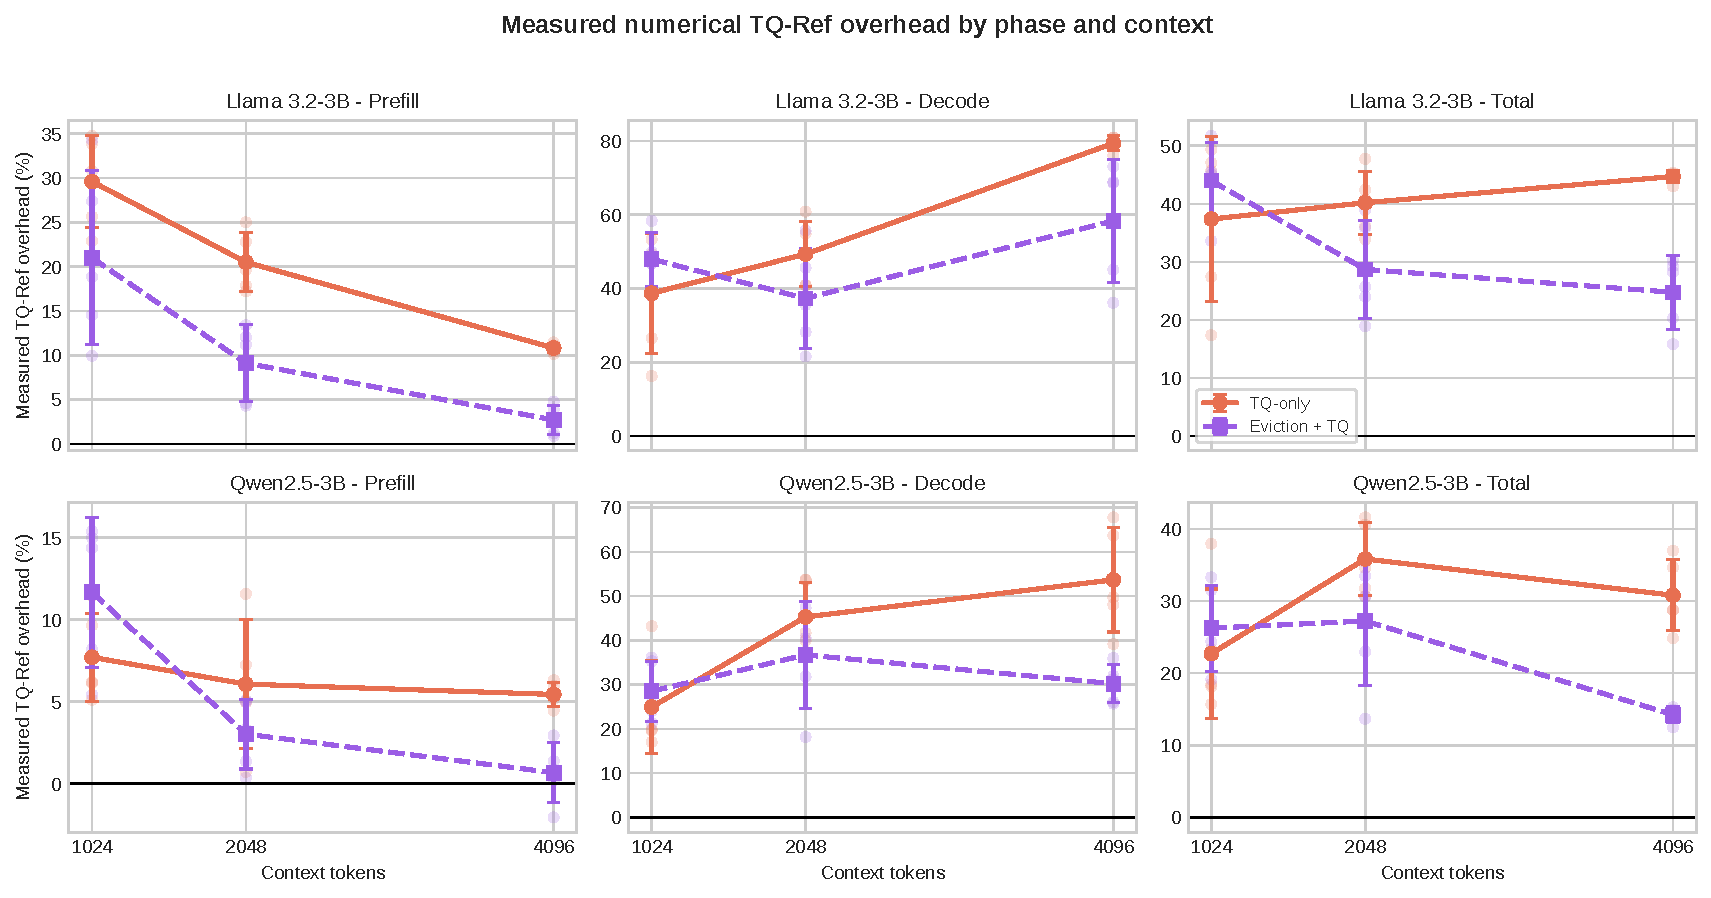
\includegraphics[width=\textwidth]{figures/fig01_measured_tq_overhead.pdf}
\caption{Measured TQ-Ref energy overhead (\%) across prefill, decode, and total inference for both models at 1024, 2048, and 4096 tokens.}
\label{fig:tq-overhead}
\end{subfigure}\hfill
\begin{subfigure}{0.48\textwidth}
\centering
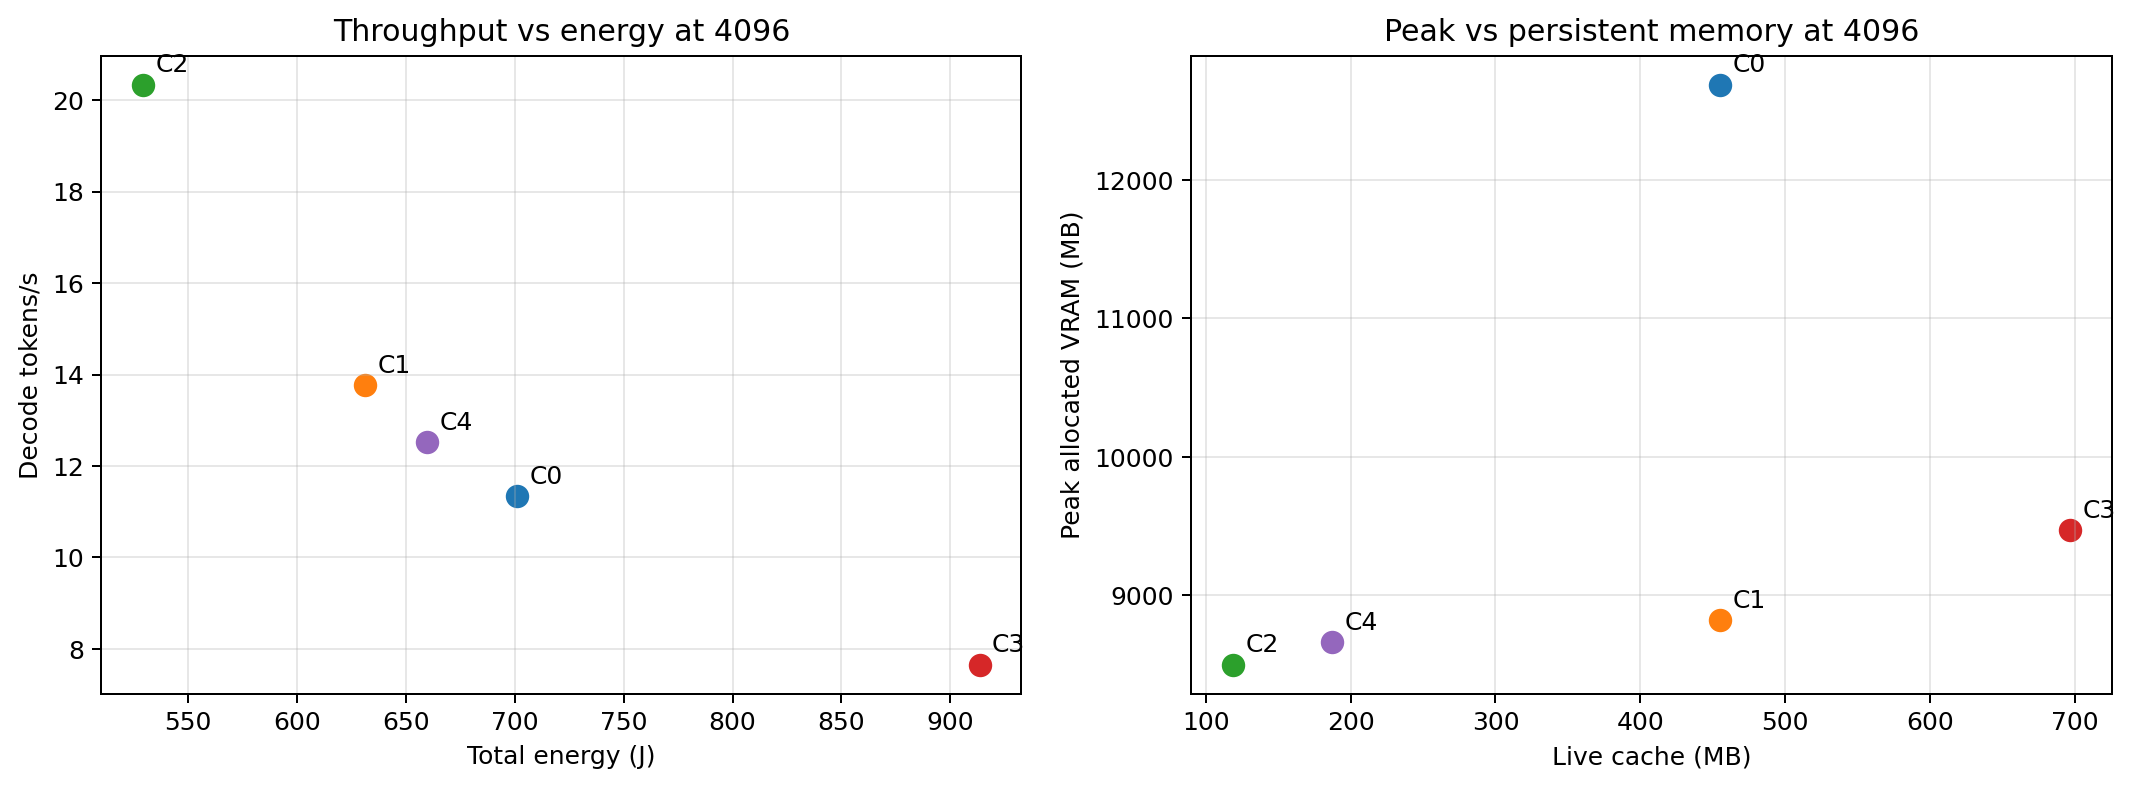
\includegraphics[width=\textwidth]{figures/v5_final_system_tradeoffs_4096.png}
\caption{System trade-offs for Llama at 4096 tokens (left: throughput vs.\ energy; right: peak VRAM vs.\ active cache volume).}
\label{fig:tradeoffs}
\end{subfigure}

\vspace{3pt}
\begin{subfigure}{\textwidth}
\centering
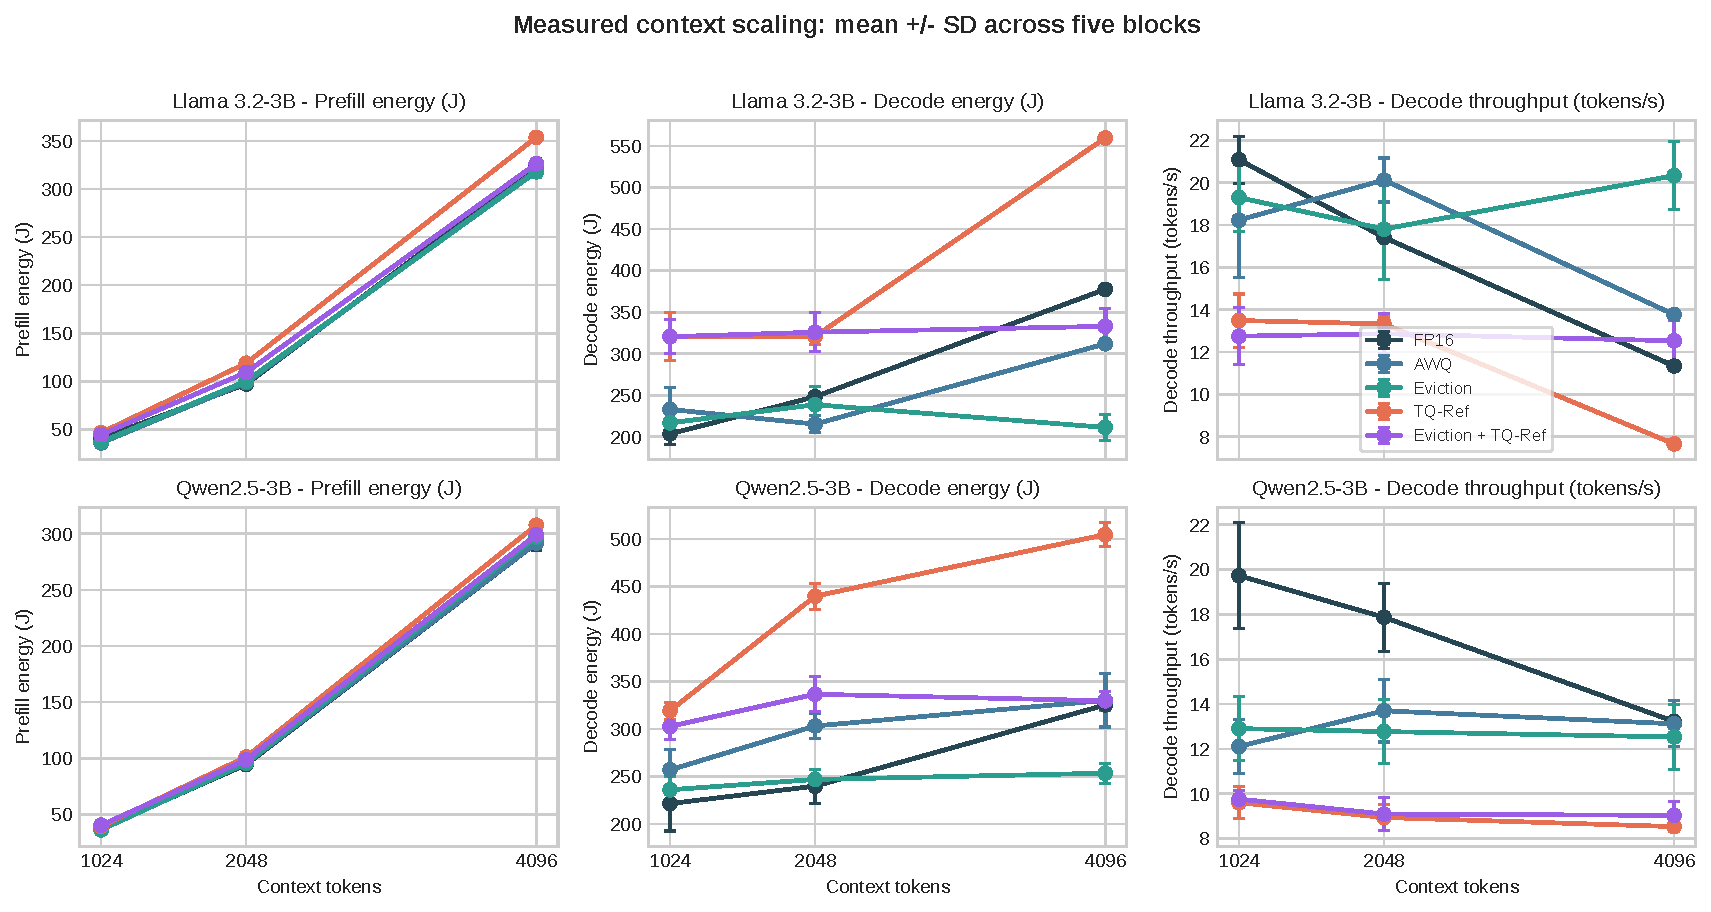
\includegraphics[width=0.75\textwidth]{figures/fig02_measured_context_scaling.pdf}
\caption{Context scaling of prefill energy, decode energy, and decode throughput across context lengths.}
\label{fig:context-scaling}
\end{subfigure}
\Description{Supplementary system measurements showing phase overhead, trade-offs, and context scaling.}
\caption{Supplementary context scaling and system trade-offs. Panel (a) breaks down phase-specific quantization overhead; panel (b) maps throughput and memory trade-offs; panel (c) shows scaling curves across context lengths.}
\end{figure*}

%% ════════════════════════════════════════════════════════════════
%%  APPENDIX C: POWER SAMPLES & CLIPPING ROBUSTNESS
%% ════════════════════════════════════════════════════════════════
\section{NVML Power Trace Distribution and Robustness Capping}
\label{app:power-samples}

Figure~\ref{fig:power-samples} shows the per-condition maximum NVML power samples across all experimental runs. The highest observed transient reading was 124.5~W on Llama and 116.1~W on Qwen. Figure~\ref{fig:power-cap} confirms that total energy rank orderings and all registered statistical significance decisions remained completely invariant when reintegrated under 82~W and strict 70~W power caps.

\begin{figure*}[htbp]
\centering
\begin{subfigure}{0.48\textwidth}
\centering
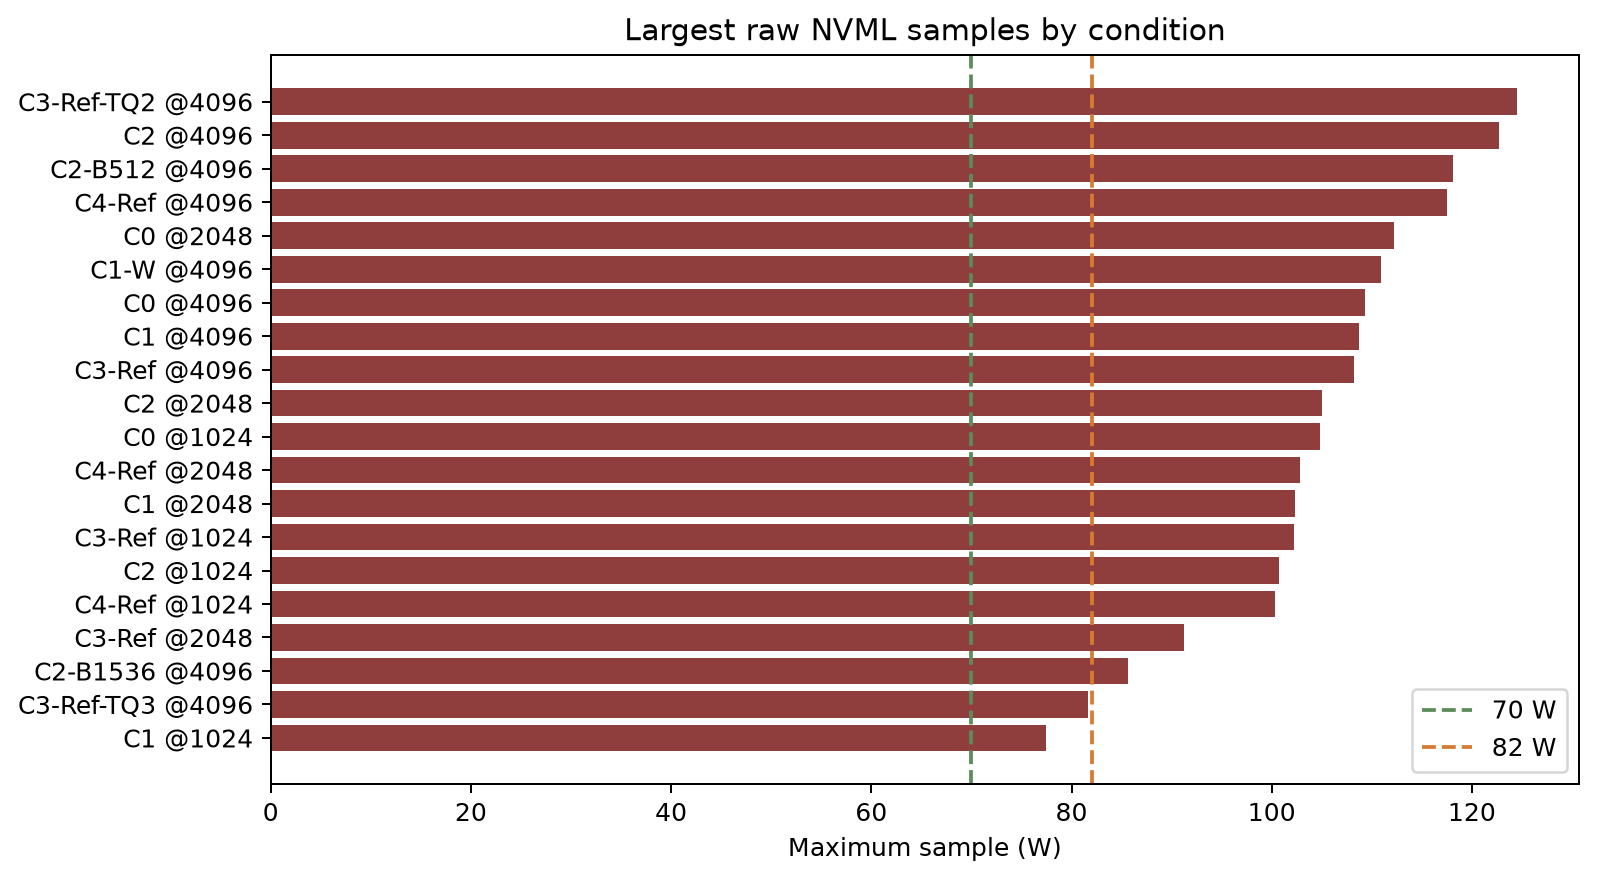
\includegraphics[width=\textwidth]{figures/maximum_power_samples.png}
\caption{Maximum NVML power samples recorded by condition.}
\label{fig:power-samples}
\end{subfigure}\hfill
\begin{subfigure}{0.48\textwidth}
\centering
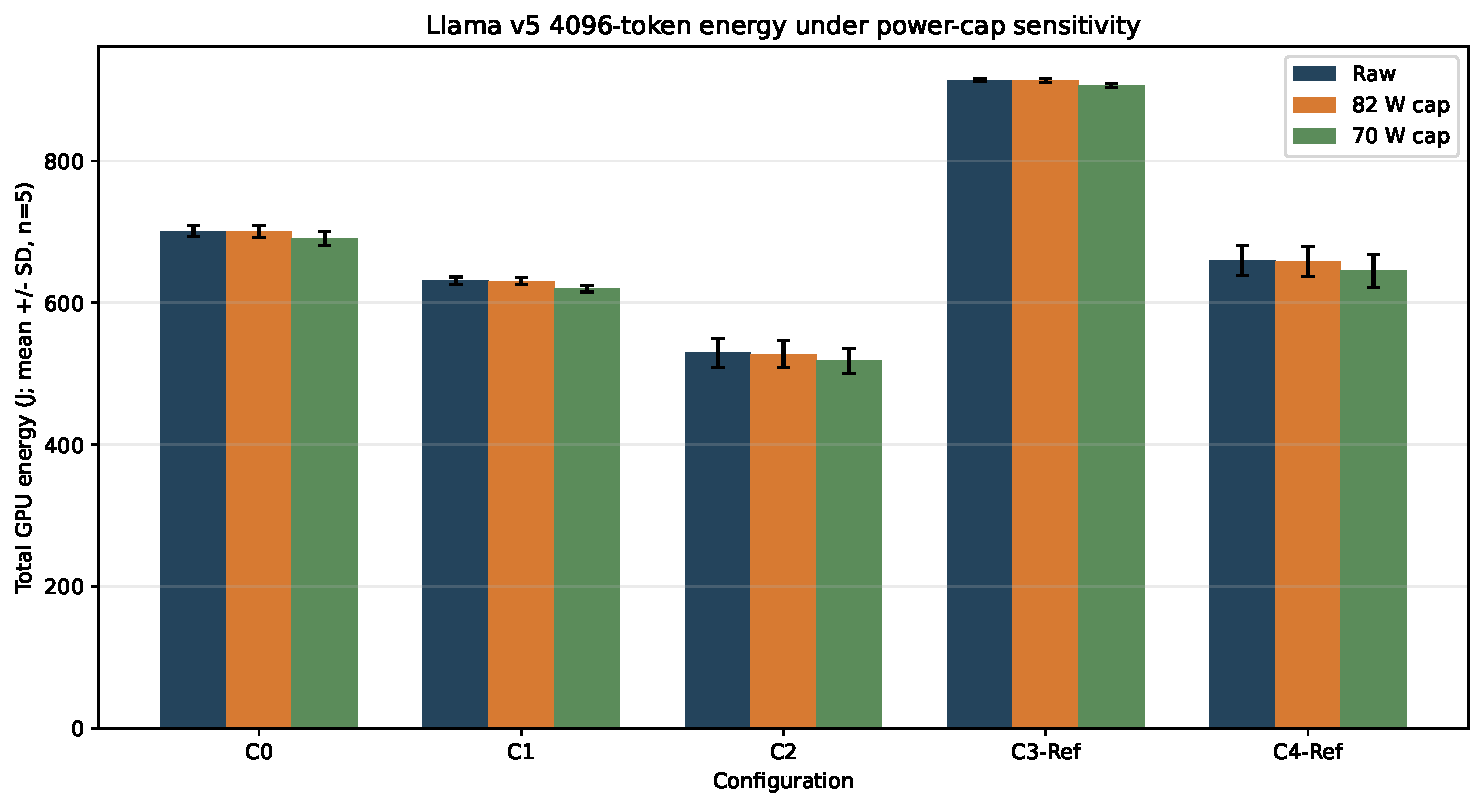
\includegraphics[width=\textwidth]{figures/core_4096_power_cap_robustness.pdf}
\caption{Total GPU energy under raw, 82~W-clipped, and 70~W-clipped integration.}
\label{fig:power-cap}
\end{subfigure}
\Description{Power trace sample distributions and clipping robustness.}
\caption{Power measurement robustness. Panel (a) plots the distribution of peak power samples; panel (b) shows stability of energy rankings under power trace clipping.}
\end{figure*}

%% ════════════════════════════════════════════════════════════════
%%  APPENDIX D: BENCHMARK CALIBRATION & RETRIEVAL SENSITIVITY
%% ════════════════════════════════════════════════════════════════
\section{Benchmark Calibration, Retrieval Confidence, and Pilot History}
\label{app:benchmark-pilots}

Figure~\ref{fig:wilson} visualizes retrieval pass rates with Wilson 95\% confidence intervals across both models, and Figure~\ref{fig:sensitivity} illustrates Llama sensitivity to eviction budget and quantization bit width.

\subsection{Pilot History and Diagnostic Headroom Progression}

To establish a diagnostic benchmark capable of detecting compression degradation without masking differences through ceiling or floor effects, we evaluated four iterative pilot configurations on Llama 3.2-3B prior to freezing the primary experimental protocol:

\paragraph{Pilot V1 (48 Records): High Distractor Density.}
The initial design placed the target needle among 48 structured records sharing overlapping key naming conventions. Both the uncompressed AWQ baseline (C1-W) and pyramidal eviction (C2) achieved 6/12 (50.0\%) accuracy. Dense lexical distractor overlap caused baseline extraction failures, obscuring differences between compression configurations.

\paragraph{Pilot V2 (32 Records): Persistent Distractor Confusion.}
Reducing document density to 32 records produced identical accuracy across both baseline and eviction configurations (6/12, 50.0\%). Structural overlap among candidate keys remained the dominant source of error regardless of overall record count.

\paragraph{Pilot V3 (Close Siblings): Floor Effect.}
To assess fine-grained key discrimination, we tested distractor records sharing prefixes and suffixes with the target needle. Retrieval accuracy dropped to 3/12 (25.0\%) for C1-W and 2/12 (16.7\%) for C2, collapsing to 0\% at 50\% and 90\% document depths. This severe floor effect demonstrated that overly difficult distractor sets mask compression differences by causing total baseline failure.

\paragraph{Pilot V4 (Structured Schema): Calibrated Headroom.}
The fourth iteration established unique, lexically distinct record identifiers with standardized schema formatting. Under this design, C1-W and C2 each achieved 9/12 (75.0\%) accuracy on preliminary probes. This provided the intended diagnostic headroom: the uncompressed model succeeded reliably while leaving sufficient dynamic range to register compression degradation. This specification was frozen and expanded to the 60-scenario evaluation suite utilized in all reported benchmark experiments. All exploratory pilot runs (V1 to V4) were archived and excluded from the final reported experimental results.

\end{document}
